% Template for replying to reviewer comments
%
% Author: Gertjan van den Burg (https://gertjan.dev)
% Source: https://github.com/GjjvdBurg/LaTeXReviewReplyTemplate
% License: MIT
% 
% Command usage:
%
%  - Reply: complete answer to the point raised.
%
%  - Partial reply: partial answer to the point raised. More text may be 
%    needed. Can also imply work on the paper that still has to be done.
%
%  - Todo reply: Used for discussion and/or sketching a reply.
%
%  - Need reply: Signals that a point needs to get a reply.
%
\documentclass[11pt,a4paper]{article}

\usepackage{geometry}
\usepackage[most]{tcolorbox}

% Colors
\definecolor{lightgray}{rgb}{0.9, 0.9, 0.9}
\definecolor{lightyellow}{rgb}{0.98,0.91,0.71}
\definecolor{lightred}{rgb}{0.8,0.4,0.4}

% Boxes
\newtcolorbox{replybox}{colback=lightgray, grow to right by=-10mm, grow to 
	left by=-10mm, boxrule=0pt, boxsep=0pt, breakable, before skip=10pt}
\newtcolorbox{partialbox}{colback=lightyellow, grow to right by=-10mm, grow to 
	left by=-10mm, boxrule=0pt, boxsep=0pt, breakable, before skip=10pt}
\newtcolorbox{todobox}{colback=lightred, grow to right by=-10mm, grow to left 
	by=-10mm, boxrule=0pt, boxsep=0pt, breakable, before skip=10pt}

% Counters
\newcounter{epntcnt}
\newcounter{rpntcnt}
\newcounter{revcnt}

% Environments
\newenvironment{reviewer}{%
	\refstepcounter{revcnt}%
	\setcounter{rpntcnt}{0}%
	\section*{Reviewer \therevcnt}%
}{}
% Editor environment takes an optional argument
\newenvironment{editor}[1][Editorial Decision]{%
	\setcounter{epntcnt}{0}%
	\section*{#1}%
}{}

% Reply Commands
\newcommand{\reply}[1]{%
	\begin{replybox}%
		#1
	\end{replybox}%
}
\newcommand{\partialreply}[1]{%
	\begin{partialbox}%
		Partial reply: \emph{#1}
	\end{partialbox}%
}
\newcommand{\todoreply}[1]{%
	\begin{todobox}%
		Todo reply: \emph{#1}
	\end{todobox}%
}
\newcommand{\needsreply}{%
	\todoreply{This comment needs a reply.}%
}

% Point command differs depending on the environment
\makeatletter
\newcommand{\point}{%
	\medskip\noindent%
	\def\@tmp{editor}%
	\ifx\@tmp\@currenvir \refstepcounter{epntcnt}\theepntcnt\textbf{.}  
	\else%
	\def\@tmp{reviewer}%
	\ifx\@tmp\@currenvir \refstepcounter{rpntcnt}\therpntcnt\textbf{.}  
	\else\fi\fi%
}
\makeatother

% Renew the commands for the point counters to get the formatting we want in 
% both the references and the item labels.
\renewcommand{\therpntcnt}{\textbf{\textup{\therevcnt.\arabic{rpntcnt}}}}
\renewcommand{\theepntcnt}{\textbf{\textup{E.\arabic{epntcnt}}}}

%\setlength\parindent{0pt}
\newcommand{\bft}[1]{\mathbf{#1}}

\usepackage[hidelinks]{hyperref}
\usepackage{natbib}
\bibliographystyle{abbrvnat}
\usepackage{booktabs}
\usepackage{subcaption}

\renewcommand{\thefigure}{R\arabic{figure}}
\renewcommand{\thetable}{R\arabic{table}}

\title{Reply to Reviewer Comments}
\author{Dirk Seidensticker}

\begin{document}
\maketitle

\noindent I thank the two referees for their helpful comments and advice. The revisions addressing their comments have substantially improved the paper, though none of its significant results or conclusions have changed.

At the request of the Editor, I have reorganized the manuscript to fully incorporate all comments made. The main structural changes are the following:\\

\begin{enumerate}
	\item The introduction has been reorganized.
	\item The history of research was amended for research before the fieldwork of the \textit{River Reconnaissance Project}.
	\item The itruduction was amended with a specific section on "Material culture and language" (see \label{rev1:linguistics})
	\item The section on "Refuting the 'Sangha River Interval' (SRI) Hypothesis" was rewritten following the suggestion of Reviewer 1 (see \ref{rev1:sri})
	\item A figure illustrating the spatio-temporal distribution of pottery styles along the Ubangi river was added to the discussion. This figure is based on a presentation of the authors at this years' SAfA meeting.
\end{enumerate}

The Author\\

\today.

\newpage
\begin{reviewer}
Reviewer \#1: The paper provides a comprehensive synthesis of the recent studies of the pottery finds of over 60 sites from north-western Central Africa. Even though the surveys and excavation date back to the 1980s, the pottery never received in depth attention until the author PhD thesis. This is consequently a very welcome contribution as it allows starting filling the gap between west-central Africa (Cameroon and Gabon) and the Inner Congo Basin, which received much more attention so far.

Large part of the results have been already published in Seidensticker 2021, but the paper provides a few new data, including new radiocarbon dates, and offers to non-german speakers the key results and hypothesis of the study.

I recommend the publication of the paper with the minor revisions listed below.

\noindent\textbf{Introduction}

\point The introduction should also include a presentation of the key questions the paper will present besides the results.

\reply{The introduction has been amended accordingly.}

\point It is not clear the author is rejecting the possibility of using historical linguistic to provide historical data about socio-cultural phenomenon of the past or pointing the methodological weakness of current work in historical linguistics. In any case, this part should be clarified and expanded to make the point of the author clearer.

\reply{In order to make the point of the author more clear, a specific sub-section has been added to the introduction.\label{rev1:linguistics}}

\point Radiocarbon dating

To avoid the reader to have to navigate the thousands of dates of the aDRAC database, all dates used in the paper related to the region studied should be provided as OSM.

\reply{The dates are added as supplementary data table Data S1 (see \ref{rev3:c14osm}).\label{rev1:c14osm}}

\point Fig. 2 and table 2 seem redundant with fig. 6. They could be moved as OSM and replace with fig. 6. It would also allow providing a clear graphic overview of the different pottery groups that will be discussed in the paper.\label{rev1:bayes}

\reply{The former Fig. 2 and Tab. 2 have been moved to a supplementary material document. It needs to be stressed though, that the approach presented in now Fig. S1 and Tab. S1, further confining the temporal limits of radiocarbon dated pottery styles using Bayesian phase modeling is a completely novel way for the archaeology of Central Africa. As a result, former Fig. 6 was moved into the results section (Fig. 2) to provide the chronological reference framework early in the text.}

\point Line 210: there is word(s) missing or the reference is not correctly formatted.

\reply{The references were formatted correctly.}

\point Imbonga style: for the reader not familiar with the area, an illustration of the Imbonga related pottery discussed in the section or of the Imbonga style in general would be welcomed.

\reply{The main features of Imbonga style pottery are illustrated best relying on finds from the Inner Congo Basin, published by \citet{Wotzka.1995}. The two finds from the lower Sangha river are non-typical vessels of the Imbonga style that can be compared to vessels from Iyonda and Bokele respectively. \citet[170 Fig.~84]{Seidensticker.2021e} illustrates this best. A reference to this figure and the chrono-typological plate in \citet[196 Fig.~93]{Seidensticker.2021e} were added to the text. The two vessels were added to Fig.~3, keeping in mind that these would not be representative for a 'classical' Imbonga.}

\point Line 297-300 : which study? Already published? If not, what are the arguments for the use of the drawing of a ring technique?

\reply{Reference to the published results in \citet[47--51 Fig.~13; 72--73 Tab.~13]{Seidensticker.2021e} were added. Detailed descriptions of macro-traces based on a larger sample size are pending publication \citep{Seidensticker.Submitteda}.}

\point Line 313 : the equator co-style tradition is not mentioned earlier. Please give a short description of its main characteristics.

\reply{The concept of the Equator-Co style tradition was established in the introduction. In-itself, the Equator-Co style tradition has no main characteristics as it is the combined evolutionary history off all pottery styles in the Inner Congo Basin and the 'branching-off' of regional pottery traditions from the West-tradition. The concept of pottery traditions used by \citet{Wotzka.1995}, and subsequently \citet{Seidensticker.2021e}, is based on the idea of a chronological sequence of ceramic styles that emerged out of each other and goes back to \citet{Willey.1945} and \citet{Rouse.1957}. In that, it differs from the use of the word 'tradition' within most of francophone studies devoted to pottery inventories from Central Africa \citep{Oslisly.1992,Clist.20042005,GouemGouem.20102011,NlendNlend.20132014}.}

\point Line 437-443: as there is an ongoing project on that topic, I would double check whether the author has the formal authorisation of Livingstone-Smith to publish this information.

\reply{The author reached out to A. Livingstone-Smith concerning this and gained written authorization to mention this aspect.}

\point Line 488: please explain. What is the bnfwa-nfwa decoration?

\reply{A short description and needed references for the the \textit{banfwa-nfwa} technique were added to the text.\label{rev1:banfwa_nfwa}}

\point Line 699-702: discrepancy already noted in Livingstone Smith et al. 2017, please insert the reference

\reply{The reference to \citet[98 Tab.~1]{LivingstoneSmith.2017}, included in the previous sentence, was moved at the end to the statement to signal that the discrepancy was noted by the original authors already.}

\point Refuting the Sangha River Interval

This paragraph should be reorganised to better highlight the data collected during the author's research to refute the SRI: I would start with the former hypothesis, then a summary of the data (archaeological and paleoenvironmental) available and, only after that, the discussion on how they are contradicting the SRI hypothesis.

\reply{The paragraph was re-structured according to the suggestion of the reviewer.\label{rev1:sri}}

\point Line 827-831: the author suggests that the C14 dates cannot be used to infer a continuity in pottery tradition in the Inner Congo Basin but does not discuss the other arguments that have been provided by Wotzka to suggest a continuity over the last 2000 years. Based on the new data, should the stylistic one should also be discarded?

\reply{A few further explanations on the reasoning \citet{Wotzka.1995} gives for the conceptualization of an uninterrupted sequence of pottery styles were added. These styles are not linked by major features, but by minute changes from one to the next, keeping elements of their precursors. \citet{Seidensticker.2018c}\footnote{See: \url{https://zenodo.org/record/1410517}} attempted to investigate the multitude of relationships \citet{Wotzka.1995} gives while describing each of the pottery styles relying on Allen's interval algebra \citep{Allen.1983} to visualize and formally review these connections. This research is currently ongoing.}

\end{reviewer}

\begin{reviewer}
\end{reviewer}
	
\begin{reviewer}

Reviewer \#3: The paper can be considered as an English abstract of a recent PhD presented in 2017 in German at the Tübingen University in Germany and recently edited in book form (2021).

All the fieldwork on which the study is based was conducted by M. Eggert between 1977 and 1987. Due to various reasons, though the main conclusions or hypotheses were published in the interim by Eggert in several papers (1983-1996, see references in the reviewed manuscript), it is only in 2017 we can consider the laboratory work to have been completed thanks to the PhD by D. Seidensticker who considered in some detail the pottery found, i.e., 30 to 40 years later. The current manuscript's English presentation is most welcome and should be published though with heavy editing.

An important aspect of the archaeological research conducted in the Congo Basin is that all the material has been kept and curated in Germany under the responsibility of M. Eggert and later H.-P. Wotzka, none being sent back to the Democratic Republic of Congo and the Institute of National Museums. Though raising several major ethical questions, it was a good thing as the collections were not lost or badly curated as it happened in other countries or for other collections kept in the country where fieldwork had been carried out. This bleak situation is known all around Central Africa, from north to south, in Cameroon, the CAR, Equatorial Guinea, Gabon, Congo, Angola and the DRC.

Several important methodological issues must be briefly discussed as they impact the manuscript's contents, its discussion and conclusion, its historical reconstruction:

i) The obvious fact all the fieldwork was conducted along rivers, and the surveys severely limited to their river banks covered by the equatorial forest without much work done between the rivers. This restricts what can be said about past land use and ancient demography in the surrounding forest.

ii) The figures given in the manuscript are evidence to another issue, the density of sites along rivers, also suggesting the results are of not much use to discuss ancient demography and land use. The Sangha River survey yielded 1 site every ca. 16 km, the one along the Ngoko river 1 every 10 km, the Ubangui survey gave 1 every ca. 19 km, the Lua inspection 1 every 25 km, and the Likwala-aux-Herbes examination 1 every 23 km (see pages 3-4).

iii) The basis of our knowledge from the area covered by the PhD and this manuscript thus represents according to the text read (page 4) 122 sites from which 14 features were fully excavated from 5 sites with some other features sampled or ly excavated from another 4 sites, giving way to a limited series of 27 radiocarbon dates from a few locations. To the "Eggert" series, one has to add, when needed, dates obtained from other projects on similar material (e.g., the Batalimo site in the CAR, the Inner Congo ones detailed in Wotzka 1995, or the ones from near Kisangani along the Congo River upstream from Eggert's surveys).

iv) Out of 24 new pottery styles, only a few are directly radiocarbon-dated. Figure 2 (page 7) provides a list of pottery styles dated by at least 2 reliable dates, though it also includes styles obtained previously. But knowing the entire spectrum of styles from the Congo basin, the 16 radiocarbon dated ones from the figure are only a small portion of the styles which have been proposed (see in Seidensticker et al 2021, annex 2, pottery styles: from 11 styles listed along the Ubangui River, only 1 is radiocarbon-dated (Batalimo-Maluba); from 13 styles along the Sangha River, only 3 are radiocarbon-dated (Pikunda-Munda, Ebambe, Mandombe), 1 with a single date (Mandombe). This means that from 24 styles described west of the Congo River, only 4 have radiocarbon dates associated, including 1 with a single 14C date; most of the styles is chrono-located by typology alone. Looking east of the Congo River we find the same picture: 35 styles are found of which 15 radiocarbon-dated; again, one must be aware 7 styles are with a single date.

Reviewer's comments about the various sections of the manuscript:

\point 1) The list of radiocarbon dates must be given in a table. Stating that "All dates are available via the aDRAC online repository (https://github.com/dirkseidensticker/aDRAC; Seidensticker and Hubau 2021) and thus not listed individually here." (page 6) This is not enough because it is not easy to use the repository and above all to locate a listing of the needed dates.

\reply{All dates from the River Reconnaissance Project were added as separate table and all dates listed in aDRAC form the general region are added as supplementary data table Data S1 (see \ref{rev1:c14osm}).\label{rev3:c14osm}}

\point 2) Page 9-11, the discussion about the Pikunda style, with one pit excavated at Pikunda, dated by 2 14C dates, and having 1 rim sherd of the Lusako style from the ICB and 4 sherds similar to the middle Ubangui river Ngbanja style.

How were the Lusako and Ngbanja styles determined? Excavated sites? Radiocarbon dates? See below.

\reply{The Lusako style was defined by \citet[104–-107]{Wotzka.1995} based on finds from excavations and surveys in the Inner Congo Basin. \citet[107]{Wotzka.1995} has access to the finds from the 1987 excavation at Pikunda and recognized the characteristic rim fragment. At the time, no site in the Inner Congo Basin that yielded Lusako style pottery was radiocarbon dated, thus \citet[107]{Wotzka.1995} uses the dates from Pikunda (KI-2877) as a reference for the Lusako style. The sherds tentatively associated with the Ngbanja style found in the lower spits at trench PIK~87/1 are distinct from the sherds of the Pikunda-Munda style defining the inventory of the pit. The most striking difference concerns the macroscopic fabric \citep[296 Tab.~34]{Seidensticker.2021e}. While Pikunda-Munda style pottery was produced unanimously using fine riverine clays void of macroscopically visible non-plastic particles \citep[62 Tab.~11; 69 Tab.~12; 115]{Seidensticker.2021e}, these sherds were produced using a different recipe; the matrix is more porous and coarse quartz inclusion can be observed. Their fabric is also distinct from the sherds of the Mandombe style that define the considerably younger pit that was partially excavated in upper 90~cm of trench PIK~87/1. Besides those characteristics, their decorations are also different: bigger impressions and raised ledges. The main inventory of the Ngbanja style, which could be described only provisionally in \citet[82--86]{Seidensticker.2021e} originates of survey finds along the middle Ubangi river and is thus undated. In light of the space available in the present paper, these details were omitted but are discussed in detail in \citet[82--86, 181--182, 296--297]{Seidensticker.2021e}.}

\point 3) Page 10: Pikunda-Munda pottery show considerable similarities with the Lokondola, Lusako, Lingonda and Bokuma styles, especially for its decoration but Pikunda-Munda has got round bases, the others flat bases. This is a major difference.

How were the Lokondola, Lusako, Lingonda and Bokuma styles determined? Excavated sites? Radiocarbon dates?

\reply{All mentioned pottery styles were described in detail by \citet[84--89, 104--120]{Wotzka.1995}. Brief descriptions, focusing on the chronology, were given in \citet[Data S2]{Seidensticker.2021}. For the convenience of the reviewer, these are reiterated here: The Lokondola pottery, while stylistically closely linked to the Inganda style, shows similarities to the younger styles Bokuma and Lingonda and must be considered an essentially subsequently phenomenon to the Inganda group \citep[89,94]{Wotzka.1995}. While no radiocarbon dates are available to date the Lokondola group, based on these stylistic links the Lokondola pottery is provisionally dated between the mid 1st c. BC and 4th c. AD by us. Lusako pottery is, based on stylistic reasoning, basically later than the Inganda style and contemporaneous with the styles Lokondola and Yete according to \citet[106--107]{Wotzka.1995}. The only radiocarbon sample associated with pottery of the Lusako style is a feature along the Sangha river \citep[297]{Seidensticker.2021e}. While the pit only yielded one rim fragment of the Lusako group, its inventory, which consists mainly of pottery of the Pikunda-Munda group, is dated into the 2nd c. BC to mid 3rd c. AD (KI-2877). This date is consistent with the dating \citet{Wotzka.1995} presents for the Inganda group and accepting \citet{Wotzka.1995} view that the Lusako style shall be later than the Inganda group, Lusako pottery might be placed best into the 1st to 3rd c. AD until more dates are available.	There are six radiocarbon dates associated with Lingonda pottery from the Inner Congo Basin. Thus based on the stylistic relations and derived chronological evidence, \citet[115]{Wotzka.1995} only accepts three to be representative for the Lingonda style (GrN-13076, GrN-14004, KN-4206). In general \citet[115]{Wotzka.1995} considers the second half of the 3rd to the 7th c. AD the period of the Lingonda group. The Bokuma pottery is considered to be contemporaneous to the Lingonda group \citep[120]{Wotzka.1995} and based on a single radiocarbon date from the eponymous site of Bokuma (GrN-14004), which is associated with Lingonda pottery as well, the style can be dated into the 3rd to the mid of the 6th c. AD for the time being.}

\point 4) Page 11 "The features also contained five nearly complete Pikunda-Munda bowls deposited laying on their sides."

Question: The five vessels are coming from the 3 features excavated at Munda (1 metallurgical feature and 2 pits) or from one and the same? 

\reply{The five vessels in questions \citep[Pl.~91.1--5]{Seidensticker.2021e} were all uncovered in the upper infill of feature MUN~87/2-1-1, which also contained the iron slag \citep[323 Fig.~157.A--E]{Seidensticker.2021e}. Below the infill was a fired clay lining and below that another infill, also containing multiple vessels and fragments \citep[Pl.~91.6--8]{Seidensticker.2021e}. The feature showed an intriguing and complex history of usage that was summarized in \citet[329 Fig.~163]{Seidensticker.2021e}. Unfortunately, due to the limited space in the paper, this detail were omitted.}

\point 5) Page 10 about the techniques in use by potters: drawing of a ring, similar to modern pottery making in the ICB. Is the author suggesting a very long and continuous technological tradition? Possible. Why not. Enough data to support this?

\reply{The author is currently working on unraveling this very issue in a research project entitled "Investigating Trans-Generational Training Networks in Central Africa: A Multi-Layered Analysis of Pottery Technology".\footnote{see \url{https://research.ugent.be/web/result/project/415328e7-c82b-11eb-a520-959c49981af2/details/3e004421-investigating-trans-generational-training-networks-in-central-africa--a-multi-layered-analysis-of-pottery-technology/en}} The research is devoted to investigate the collective production sequences (\textit{chaînes opératoires}) and the provenance of vessels to infer communities of practice and their interrelationships through time. Early results from that project indicate that certain aspects of the \textit{chaîne opératoire} persist for quite some time. Thus, for the time being the author would need to give a negative answer to this question, as research on that topic only commenced recently.\label{rev3:pottery_tech}}

\point 6) On page 12 the introduction to an Early Iron Age is confusing. We read about the northern Congo basin (i.e., the Ubangui river) that "three distinct regional lines of development" exist. Only one is presented, from the lower part of the river, and "Inventories from sites in that region are dominated by the newly described Bokwango style and the already established styles Bondongo, Mbandaka, and Botendo (Seidensticker 2021, 96-98, 172-181). All these groups are dated into the late Iron Age." We jump from the EIA to the LIA. From the reviewer's understanding something is missing in this section.

\reply{The introduction was changed to highlight only those groups pertaining to the Early Iron Age.\label{rev3:eia_nCB_intro}}

\point 7) About the survey along the Ubangui river (page 3): "only the site of Motenge-Boma has been known previously (van Noten 1977, 1982, 75)." Better to speak of published sites. Others were known through surface collecting but were kept in archives as in the Africa Museum in Belgium (DRC), or the Musée de l'Homme in France (Congo and the CAR).

Was there any time a check carried out on the collections kept in Paris and in Tervuren?

\reply{The statement has been amended. The author only checked the collections kept at Tervuren, but never those at Paris. Checking the online inventory of the collection hosted by the Musée de l'Homme (\url{https://science.mnhn.fr}) revealed no objects from Central Africa. The author will establish contact with the Musée de l'Homme.}

\point 8) Batalimo-Maluba style was found on 18 sites and are securely dated by the only two excavations, at Batalimo and by Eggert at Maluba. Using the contents of the excavated features from these sites must be the core of our understanding of the style (from page 12).

\reply{The basis of the description of the Batalimo-Maluba style in \citet[75--82]{Seidensticker.2021e} is based mainly on the findings from two pit features excavated at Maluba \citep[264--272]{Seidensticker.2021e}. Survey finds were included as second-tier. The well published description of the finds from Batalimo by \citet{Aumassip.1975} were included in the description, but those finds were not pursued and subjected to a follow-up analysis. The author knows about finds from the site of Batalimo that were uncovered by \citet{Ndanga.2010} hosted at the RMCA Tervuren. These are very similar to the ceramics published by \citet{Aumassip.1975}, \citet{Eggert.1987c}, and lately \citet{Seidensticker.2021e}, with some sherds also showing characteristics more reminiscent of the Ngbanja style.}

\point 9) Regarding the second component proposed about the EIA from the northern past of the Congo basin, i.e., the Ubangui river, we have the Ngbanja style (page 14). It "shares similar general characteristics" with the Batalimo-Maluba style, though it is also stated it is "strongly related to the Batalimo-Maluba style" to the point Eggert had posited it could be an early development of the coming Batalimo-Maluba style.
About the chronology of the Gbanja style: "the only chronological fixpoint for the Ngbanja style is a sherd of this style found in the deep pit at Pikunda. ". On pages 9-11 Ngbanja style pottery is represented by 4 sherds in one pit from Pikunda. So much as further down in the text it is stated was found "Three other sherds with coarse fabric and a decoration different from the Pikunda-Munda style were also found". It makes 4 sherds, but why write about 4 Ngbanja sherds further up? To be corrected.
The chronology of this Ngbanja style must be taken with caution: a single sherd in a pit dated twice to ca. 1884 cal BP (KI-2877, 1980+/-100 bp) and ca. 1734 cal BP (RICH-30864, 1850+/-24 bp).
How can we relate one sherd in a dated feature to a style defined by a series of surface finds?
Is the Ngbanja style truly different from the Batalimo-Maluba style?

Looking at the Ngbanja style pottery there is some similarities, especially for illustrated specimen n°2-5 (Seidensticker 2021 edited PhD, Abbildung 26, page 83); but then Ngbanja pottery would be round based when Batalimo-Maluba pots are flat based and Pikunda Munda sometimes flat but mostly convex? All pottery with extended or full profiles are from the surface?

Looking at the find maps (Seidensticker 2021 edited PhD, Abbildung 27, page 85), the reviewer is surprised to see the sites where Ngbanja sherds were found are located on the Sangha river (4 of them) in Pikunda-Munda "territory", the western Congo basin, and along the Ubangui river (2 of them), not concentrated on the latter river, inside the northern Congo basin.

Why not consider Ngbanja is rather related to Pikunda-Munda?

\begin{figure*}[!tb]
	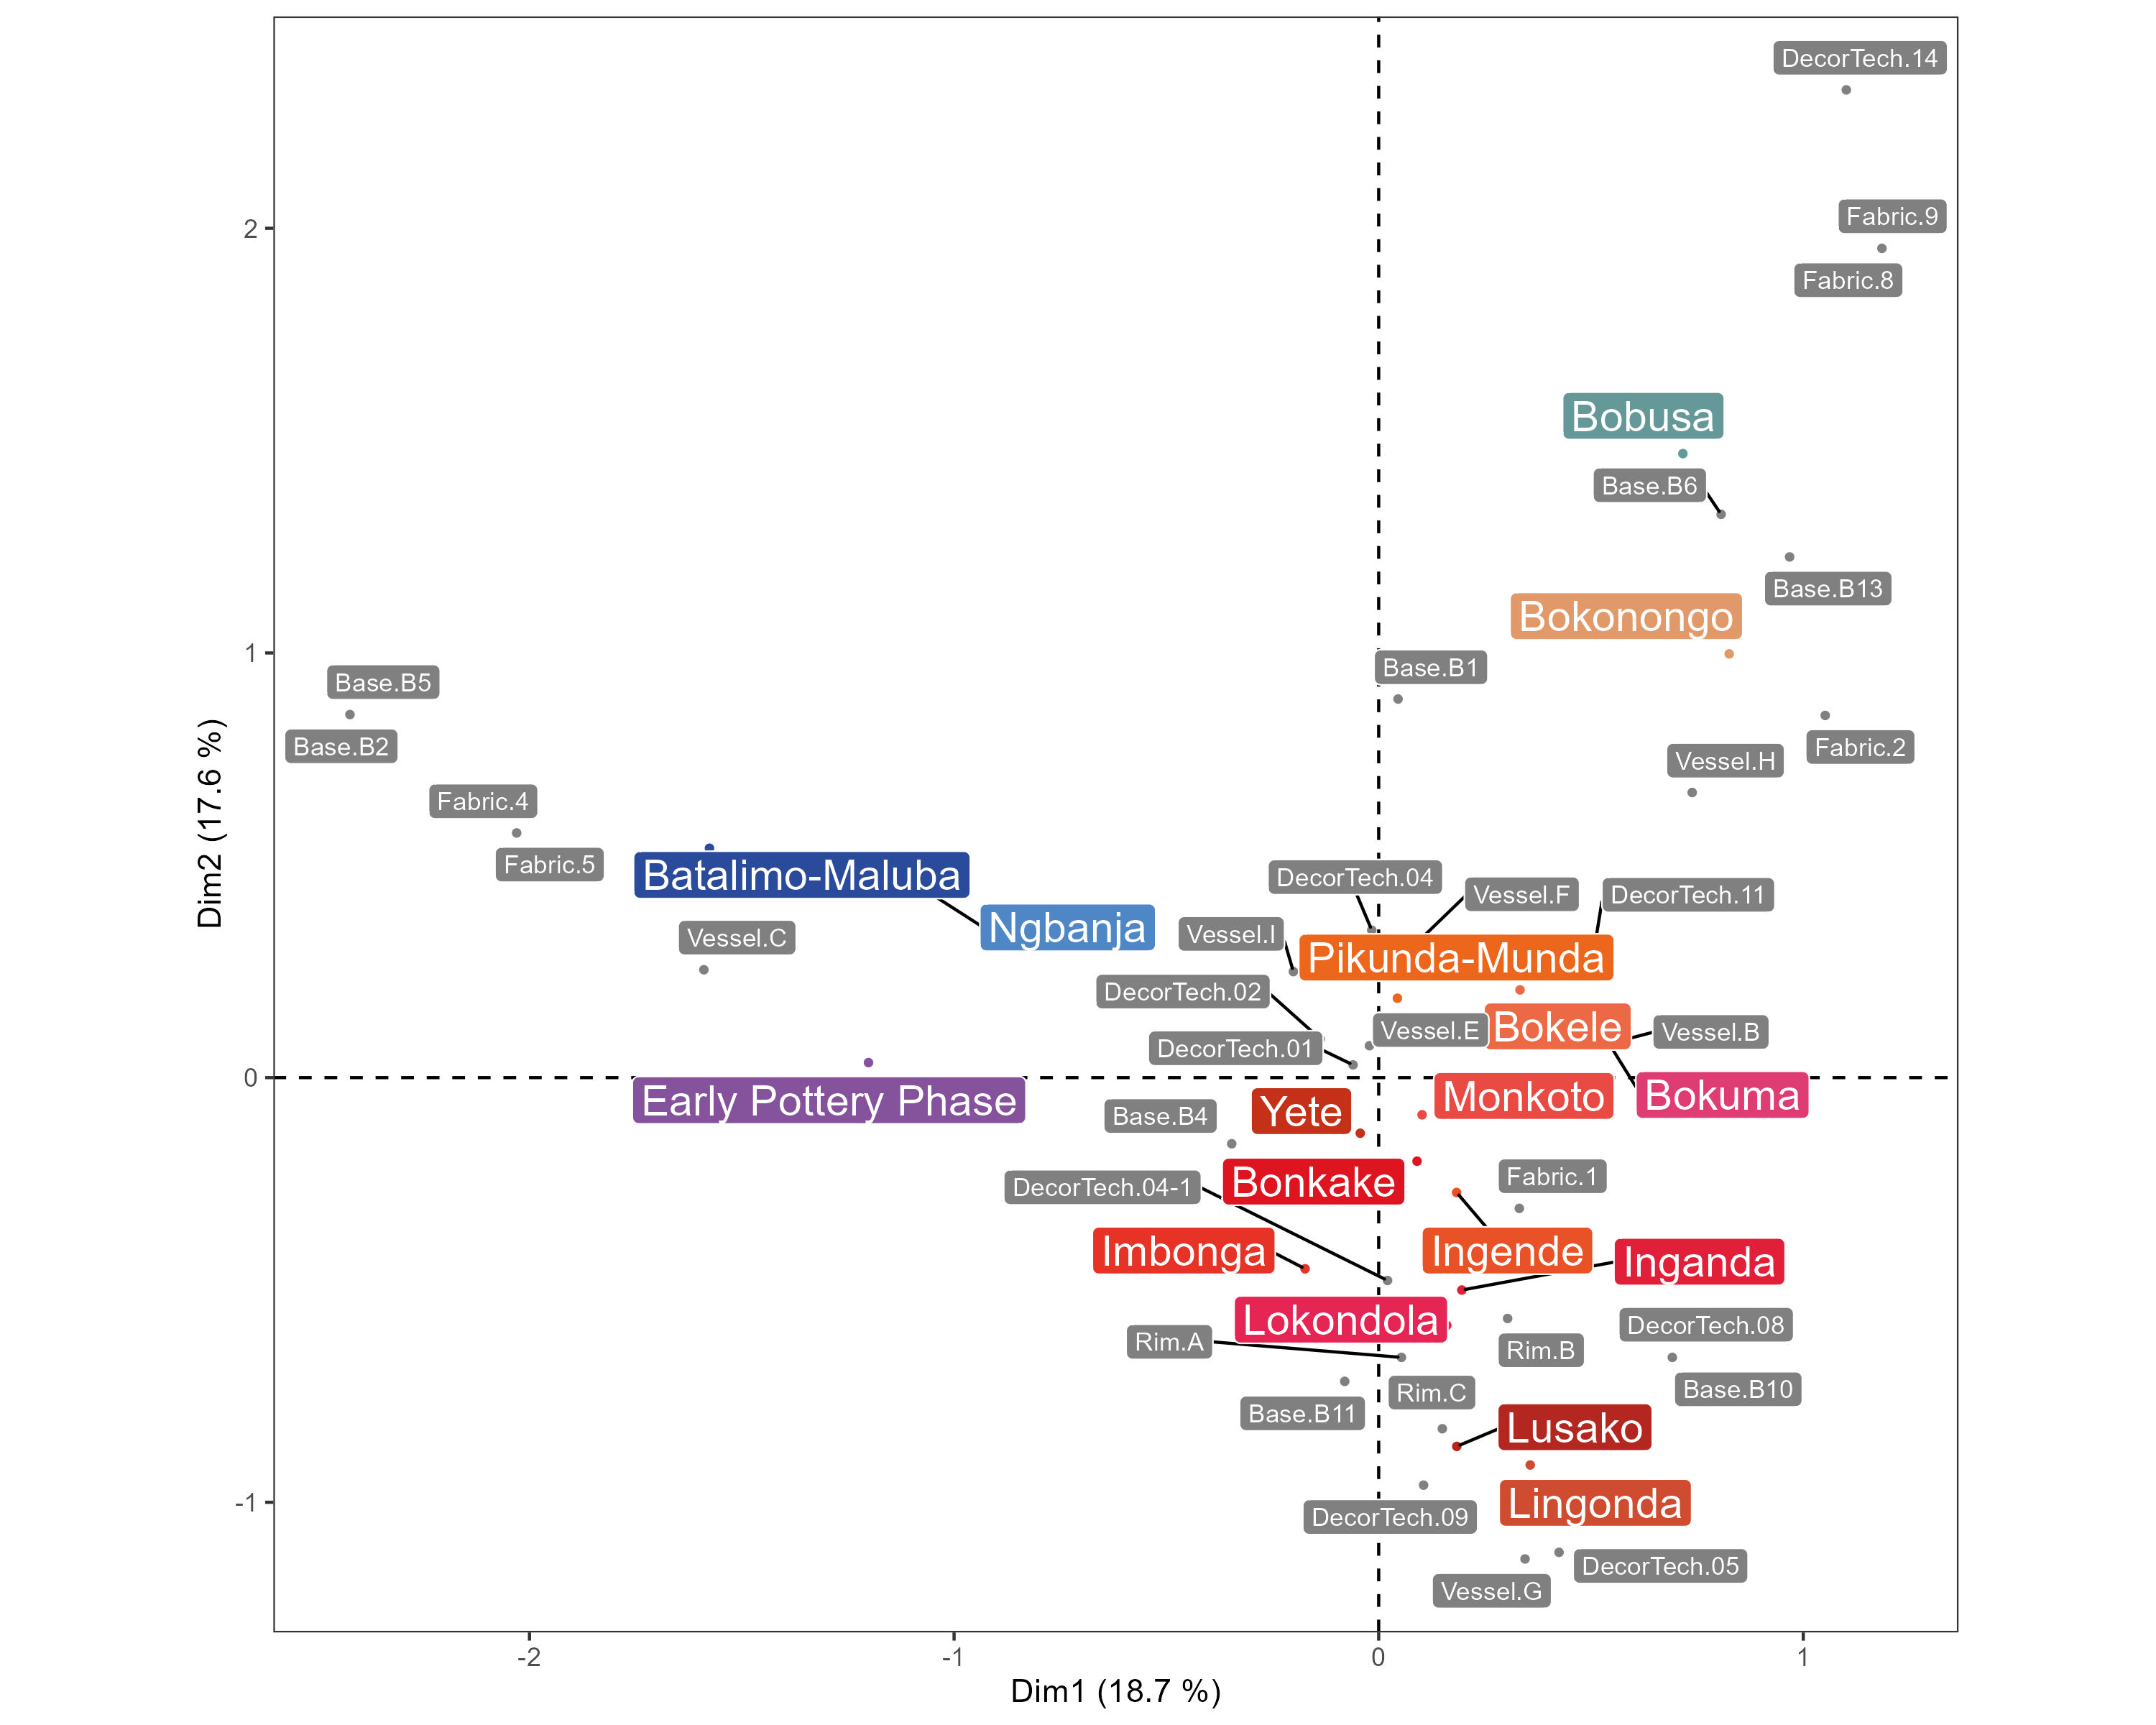
\includegraphics[width=\textwidth]{fig/varia_potterystyles_eia_attributes_ca.jpg}
	\caption{Correspondence analysis of attributes of pottery groups dating into the Early Iron Age from the Congo Basin, 1st and 2nd eigenvectors. Attributes recorded are encoded in reference to \citet[30 Fig.~5: vessel types; 32 Fig.~8: shape of the rims; 33 Fig.~9: shape of the base; 36--38 Tab.~7: decoration technique; 62--65 Tab.~11: fabrics]{Seidensticker.2021e} and displayed in gray. Typology of vessel and rim shapes from the Inner Congo Basin as described by \citet{Wotzka.1995} has been mapped to the systematic developed for the northern and western Congo Basin \citep[30 Fig.~5: vessel types; 32 Fig.~8: shape of the rims]{Seidensticker.2021e}. Comparison tables can be found at the online repository aSCAC (\textit{Archive des styles de céramique en Afrique centrale}; \url{https://github.com/dirkseidensticker/aSCAC}).}
	\label{fig:potterystyles_eia_attributes_ca}
\end{figure*}

\reply{The author is deeply involved in approaching the underlying issue of this remark, i.e. how can we define closeness between pottery styles. To date, archaeological approaches to this issue are mainly based on individual interpretations of distinct criteria and profoundly subjective. An example of such an approach can be seen in the examination of the decorated parts of vessel of the Imbonga style by \citet[750 Tab.~8-11]{Clist.20042005}. The authors is currently working on applying multivariate statistical techniques that are standard practice in ecological research \citep{Borcard.2011,Legendre.2012}. These procedures, including correspondence analysis, are robust methods for finding and displaying relationships between categorical variables (type presence-absence). The potential of this approach within archaeological research is evident \citep[cf.][]{Muller.2015}. As a precondition, the properties of pottery styles included will have to be encoded within a unified system.\footnote{see: \url{https://github.com/dirkseidensticker/aSCAC/blob/master/potterygroups_attributes.csv}} A baseline for this can be the typology described for the northern and western Congo Basin \citep[27--39]{Seidensticker.2021e}. The properties of pottery styles from the Inner Congo Basin are described in detail by \citet[56--210]{Wotzka.1995}, using a very detailed typology. In terms of vessel shapes, \citet{Wotzka.1995} encoded 115 individual types. For a diachronic comparison of these types throughout the last two-and-a-half millennia, the 115 individual vessel types were mapped against the more generalized system of the northern and western Congo Basin.\footnote{see: \url{https://github.com/dirkseidensticker/aSCAC/blob/master/Wotzka1995-Seidensticker2021_VesselTypesConcordance.csv}}. Similarly, the 211 individual rim types used by \citet[435--439 Pl.~1--5]{Wotzka.1995} were mapped onto the basic types described in \citet[32 Fig.~8]{Seidensticker.2021e}.\footnote{see: \url{https://github.com/dirkseidensticker/aSCAC/blob/master/Wotzka1995-Seidensticker2021_RimTypesConcordance.csv}}. Regarding the Ngbanja style in question, a preliminary analysis of the multi-variate co-dependencies of attributes of pottery styles from the Congo Basin dating into the Early Iron Age, which also included the properties of the Early Pottery Phase of the north-eastern Congo Basin as described in \citet{LivingstoneSmith.2017}, corroborates the relatedness of the Ngbanja and Batalimo-Maluba styles (Fig.~\ref{fig:potterystyles_eia_attributes_ca}). The bi-plot of the 1st and 2nd eigenvector shows the similarities of pottery styles pertaining the West-tradition of the Equator-Co style tradition (shown in different shadings of red) that are clusting close by each other. The Ngbanja pottery is set apart from this cluster and closer to the Batalimo-Maluba style and the Early Phase pottery of the north-eastern Congo Basin than it is to the styles of the Inner Congo Basin. While the only date associated with pottery of the Ngbanja style comes from the Pikunda-Munda pit feature at Pikunda, the few sherds related to the Ngbanja style are clearly outliers in that inventory, accounting for only 2.4~\% of sherds \citep[296--297 Tab.~34--35]{Seidensticker.2021e}. Thus, the author feels confident in the association of the Ngbanja pottery with the Batalimo-Maluba group. Approaching this issue using multivariate statistics is still ongoing, thus the presented results in Fig.~\ref{fig:potterystyles_eia_attributes_ca} here have to be seen at preliminary.\label{rev3:ngbanja}}

\point 10) A Middle Iron Age does not exist. No sites dated between 500 and 1000 CE (page 14).

Using the data from the Kisangani area to bolster the claim is not possible (page 14). The very interesting results from there is preliminary. We have only 10 14C dates, correctly grouped into an Early, a Middle and a Late pottery phase (Livingstone Smith et al. 2017, fig. 23, page 17). Fig. 6 page 22 of the present manuscript show for Kisangani a rather continuous occupation throughout the period.

How can we think we jump from an Early Iron Age to a Late Iron Age? See our fourth preliminary remarks about still undated pottery styles.

\reply{The header was ambiguous and was amended to "Hiatus (500--1000 CE) in the Congo Basin" to reflect the issue more clearly. The impression of a continuous occupation in the Kisangani area in Fig.~2 (former Fig.~7; see \label{rev1:bayes}) is distorted by the two dates associated with Ilambi style pottery and their deviation: while one date covers the 8th to 10th c. CE (Poz-75462) the second one dates into the 15th to 17th c. CE \citep[Poz-75451;][98 Tab.~1]{LivingstoneSmith.2017}. For the time being no decision on the correct time-span of the Ilambi pottery can be given. No radiocarbon dates are associated with the other pottery style of the later phase, the Yaekela style. Reviewing the available radiocarbon dates and the issue on a bigger scale reveals a prominent bi-modal pattern \citep[Fig.~2]{Seidensticker.2021}: dates associated with the Early Iron Age are clearly separated from those associated with the Late Iron Age. This 'hiatus' was first discussed by \citet[101--103]{Oslisly.1998} and \citet[171--172]{deMaret.2003}.}

\point 11) Stating that a pattern of putative demographic changes in Central Africa during the past three millennia is firmly established by two published papers is exaggerated and misleading. The author does not at least mention nor discuss opposite views, or rather that the data at hand, i.e., less radiocarbon dates within a period, can be understood other ways than his.

See the recent paper Clist (B.), Denbow (J.) \& Lanfranchi (R.), 2023, Using the radiocarbon dates of Central Africa for studying long-term demographic trends of the last 50,000 years: potential and pitfalls, Azania: Archaeological Research in Africa, 28(2), pp. 235-293.

To be added to the references.

\reply{The author is aware of the recent publication by \citet{Clist.2023a}, which was published after the submission of this manuscript. As far as the data from the western Congo Basin are concerned, the author notes a severe misrepresentation of the data by \citet{Clist.2023a}. Data from the study area of the present paper are listed in \citet[39 Tab.~7]{Clist.2023a}, which’s caption is erroneous as only the site of Pikunda is situated along the Sangha river; Maluba is along the Lua river and Munda on the Likwala-aux-Herbes river. In order to claim that the known issue with dates measured at the radiocarbon dating laboratory of Hannover during the 1980s \citep{Geyh.1990} are insignificant, \citet[37--39]{Clist.2023a} utilize un-calibrated radiocarbon dates only and de-contextualized the data. Calibrating the data, some of which have substantial standard errors of more than 100 years, clearly shows that they statistically overlap at 2$\sigma$ \citep[268 Fig.~112; 320 Fig.~155; 328 Fig.~162; 334 Fig.~167]{Seidensticker.2021e}. The two dates obtained from bone material from feature MLB~87/1-4-3 are overlapping peripherally at 2$\sigma$ after calibration with IntCal20 \citep{Reimer.2020}, which was not the case using IntCal13 \citep[277 Ftn.~357]{Reimer.2013,Seidensticker.2021e}. A severe contortion of the data concerns the two dates \citet[39 Tab.~7]{Clist.2023a} list from Pikunda (KI-2891, KI-2877): While they were obtained in the same trench (PIK 87/1), they do not pertain to the same feature \citep[121 Fig.~6.4]{Seidensticker.2016b} \& \citep[299 Fig.~138, Tab.~36]{Seidensticker.2021e}. KI-2891 dates a pit whose infill is characterized by Mandombe style pottery and that reaches down to 0.95~m below the surface and cuts into the infill of a 3.6 m deep pit with pottery of the Pikunda-Munda style. The two samples were taken in spits about 95--105~cm apart from each other. Thus the falsely argued difference between the dates by \citet[39 Tab.~7]{Clist.2023a} is an irrefutable result of the archaeological context. It is striking how \citet[1]{Clist.2023a} can claim that "each date has been checked for their context" and advocating for a predominant study of the 'context' \citep[4--5,20,29--30,37--39]{Clist.2023a} when a quick review, as the one presented here, reveals severe issues with their handling of data. Furthermore, \citet[29--30]{Clist.2023a} conceal the approaches on classifying radiocarbon dates according to criteria of 'chronometric hygiene' \citep{Spriggs.1989,Spriggs.1993,Pettitt.2003,Napolitano.2019} by \citet[9,Tab.~S1]{Seidensticker.2021}. It is important to note, that \citet{Seidensticker.2021} not simply removed not representative dates, such as the two dates from Otoumbi 2 that \citet[29]{Clist.2023a} mention, but marked those in a transparent system \citep[9]{Seidensticker.2021}. Only during the statistical analysis \citep{Seidensticker.2020b} are dates retained that are deemed representative for human activity as explained in detail \citep[9--10]{Seidensticker.2021}. This transparent classification system for the radiocarbon dates is not only a cornerstone of the study by \citet{Seidensticker.2021} but also completely novel for the region. Neither \citet{deSaulieu.2021a}\footnote{The data from \citet{deSaulieu.2021a} have been published online independently \citep{deSaulieu.2021}.} nor \citet{Clist.2023a} provide a classification system even closely as transparent as \citet[9,Tab.~S1]{Seidensticker.2021}. In consequence, the author fails to see an "opposite view" on the "pattern of putative demographic changes in Central Africa" in the paper by \citet{Clist.2023a} as this studies conclusions are impaired by a) a lack of calibration of data, b) negligent handling of contextualization of data, and c) concealment of approaches to contextualize data by \citet{deSaulieu.2021a} and \citet{Seidensticker.2021}. Viable approaches to testing for representativity can be based on formal modeling \citep{Galletti.2013,Gillespie.2016,Jones.2019,AlwiMuttaqin.2019,Boemke.2023}. The "influences of the presence or absence of sites" can be studied "based on the maximum entropy principle developed for species distribution and environmental niche modeling" \citep{Phillips.2008,Phillips.2009,Phillips.2017}.\label{rev3:clist}}

\point 12) The reviewer believes the problem identified in our point 6 about page 12 finds its solution here on page 15, in the first paragraph under Late Iron Age. He thinks the two other distinct regional lines of development are here. If correct the two sections must be edited into one.

\reply{To keep the general diachronic focus of the paper, the reference to younger styles in the introduction of the Early Iron Age in the northern Congo Basin (see \ref{rev3:eia_nCB_intro}) has been removed. It is a key aspect of this paper to regard the chronology as first-tier element, while the different regional lines of development are considered second-tier.}

\point 13) We need a map of the Late Iron Age styles mentioned: Ngombe, Ebambe, Epena, but also about the Ngoko Tradition. The reviewer cannot fathom the geographical distribution.

\reply{In restructuring the former Fig. 7 (see \ref{rev3:distr_fig}), the distribution of these two styles can be retraced better on now Fig. 6. The author would refrain from simply reproducing existing distribution maps in \citet[136 Fig.~59, 140 Fig.~62]{Seidensticker.2021e}.}

\point 14) Page 16: What is a bnfwa-nfwa décor? Please description and if felt as important an illustration is needed.

\reply{A short description and needed references for the the \textit{banfwa-nfwa} technique were added to the text (see \ref{rev1:banfwa_nfwa}).}

\point 15) Again, page 17, we find an approach to dating pottery based on the typology without any 14C dates. The Ngoko Tradition is made out from 5 styles or groups, only 2 being dated. The author putting together his way of looking at pottery with a few radiocarbon dates can write: "The proposed order of these pottery styles starts in the 13th to 15th century CE with the Mandombe style, followed by the Kondo group and the Ouesso group, which in turn are surpassed by the Pandama style, which links to the modern Mbenja pottery". This rapid succession of the use of 'style' and 'group', knowing a 'group' is made up of several 'styles', is confusing.

\reply{It must be noted that, unlike the impression the reviewer got, the term 'group' is simply used as synonym for 'style' and thus a 'group' is note made up of several 'styles'. Observed succession of one style into another is systematized as 'style tradition', as is the case with the 'Ngoko style tradition'. A preamble explicitly stating that 'group' is used synonymous for 'style' is introduced in the materials and methods section.}

\point 16) Page 19. Speaking of the Eastern Congo Basin regarding the finds west and east of Kisangani, on the Congo River, cannot be considered accurate but rather misleading. See figure 1 in Livingstone-Smith et al. 2017 where it is evident, we still have nothing done in the true eastern Congo basin. The finds reported in 2017 lie north-east of the finds of Eggert, but still associated with the Inner Congo Basin. When we will sometime excavate in the east we would have to call the area the "far east".

\reply{The references to the region around Kisangani was harmonized to 'north-eastern Congo Basin' as this term was already used in other parts of the text.}

\point 17) The section entitled "Late Iron Age (1000-1850 CE) in the Northern Congo Basin" pages 18-19 are illustrative of the poor knowledge we have of that area, with most of the pottery found from the surface (jump to the conclusions where the author says so). I fear another way to look at the Western Congo Basin would lead to a similar picture.

\reply{The lack of excavated features and thus reliable archaeological contexts in the northern Congo Basin, i.e. along the rivers Ubangi and Lua, is considerable. During the \textit{River Reconnaissance Project} excavations were only carried out at one site and those yielded mostly features defined by pottery of the Batalimo-Maluba style. But layers on top of the two main pit features MLB~85/1-3-1 and MLB~85/1-3-2 as well as one incomplete excavations of a pit at Maluba \citep[279]{Seidensticker.2021e} yielded isolated sherds representing the younger phase of the sequence. The archaeological record of the western Congo Basin, while not as comprehensive as one would wish, is considerably more encompassing. In total 14 features \citep[Cat.-No. 6--19]{Seidensticker.2021e} were studied, representing the early as well as later parts of the sequence. It is undisputed though that new fieldwork will further expand on the fragile knowledge we have of the communities that lived in the Congo Basin during the past more than two millennia.}

\point 18) Page 20, it should be stated that during the time of the Imbonga Group, pottery using communities show up around Kisangani before the development of the Balatlimo-Maluba and Pikunda-Munda pottery-using villagers. The paragraph(s) about Kisangani should be moved upward from an historical point of view.

Reference to the Ngbanja style should be removed as explained earlier. Linking the Early Phase pottery of Kisangani whose early trace is in years BC to the Ngbanja style, surface collected and possibly dated to after the start of the CE, is stretching the data too far.

\reply{The paragraph on the north-eastern Congo Basin was moved up as suggested by the reviewer. Concerning the putative relation of the Ngbanja style pottery to the ceramics of the Early Phase in the north-eastern Congo Basin, the author amended the basic argument in the comment above (see \ref{rev3:ngbanja}). For the sake of this paper, the author refrained from 'stretching the data too far' and removed the reference to the Nbganja style.}

\point 19) Page 21. "Within the entire Congo Basin, only very few sites point to the presence of pottery-producing communities between the 7th to 10th centuries CE". It is better to write "only very few dated sites". We know nothing of all the undated styles which exist.

As a reminder, see our preliminary note IV, out of 59 pottery styles west and east of the Congo River, only 4 have radiocarbon dates associated, including 1 style with a single 14C date, to the west, and to the east we have only 15 styles radiocarbon-dated, again with 7 of them with a single date. Overall, we can only chrono-locate safely 11 pottery styles, 3 to the west and 8 to the east of the Congo River.

Looking at figure 6 for the Northern, Western and the Inner Congo Basin (a Central Congo basin?), one should remove all the styles marked by squares because they depend on the acceptance of typology-based dating which cannot be deemed safe.

\begin{table*}[!tb]
	\centering
	{\small \begin{tabular}{lrrrr}
		\toprule
		\textbf{Region}      & \textbf{Radiocarbon} & \textbf{\begin{tabular}[c]{@{}l@{}}Ethnographic\\\textit{Terminus ante quem}\end{tabular}} & \textbf{\begin{tabular}[c]{@{}l@{}}Relative\\Chronology\end{tabular}} & \textbf{Total} \\
		\midrule
		Northern Congo Basin & 1 (9\%) & 4 (36\%)  & 6 (55\%) & 11 \\
		Western Congo Basin  & 6 (40\%)  & 3 (20\%) & 6 (40\%) & 15 \\
		Inner Congo Basin    & 14 (41\%) & 5 (15\%) & 15 (44\%) & 34 \\
		Eastern Congo Basin  & 3 (75\%) & 0 & 1 (25\%) & 4 \\
		\bottomrule       
	\end{tabular}}
	\caption{Ratio of dated pottery styles in the Congo Basin separated by region and by means of dating method (cf. Fig.~2). Numbers are divided in styles only known from archaeological studies that thus can only be absolutely dated using radiocarbon dating, those that are dated due to being present in ethnographic records, followed by those that are only dated by means of relative chronology.}
	\label{tab:ratio_dated_styles}	
\end{table*}

\reply{It was specified that "only very few dated sites point to the presence of pottery-producing communities between the 7th to 10th centuries CE". In tallying the dated and undated styles, the reviewer might have missed that quite a substantial amount of styles included in Fig.~2 are 'dated' relying on a \textit{terminus ante quem} derived from ethnographic records. A compilation of the ration of known pottery styles from the region shows that only in the northern Congo Basin, more than 50\% of styles are only dated my means of relative chronology (Tab.~\ref{tab:ratio_dated_styles}). While 'typology-based dating' dating, i.e. relative chronology, is indeed unsafe, it remains a suitable instrument of discussing relations between chronological entities even in the time of chronometric dating \citep[152--162]{Eggert.2012e}. The authors refrains from omitting parts of the results of this analysis and refers to the case of the Ngombe style. Due to the fact that in the late 1980s the lab in Kiel could not extract enough organic material from a sample excavated at the eponymous site \citep[305--306]{Seidensticker.2021e}, the pottery could only be dated in relation to the styles Mbandaka and Longa from the Inner Congo Basin. The proposed date, the 12th to 14th century CE \citep[128]{Seidensticker.2021e}, was perfectly corroborated by a new AMS date coming from a food crust of the main vessel found at Ngombe that dates into the late 12th to mid-13th century CE (RICH-30867). This shows that relative chronology can derive robust estimates. The present manuscript clearly marks those groups throughout the text as well as in Fig.~2. Removing these groups would give a false impression of the state knowledge. The author is convinced that, similar to the representation of radiocarbon dates (see \ref{rev3:clist}) a systemic classification and labeling of problematic data in a reproducible way serves future research better than mere omission of data.}

\point 20) Page 23 and figure 7. The same applies here. The spatial patterning uses all the known sites of the various styles, the dated and undated ones. Removing the undated styles would make things much clearer without forgetting making use of the research biases about spatial patterning demonstrated and explained in the paper already mentioned (Clist et al. 2023). The picture should be one of linear patterning as all the surveys were carried out along the waterways without any good survey inland between the rivers.

Seen another way, what is the interest in this too confusing figure? I am of the opinion it should be removed.

\reply{Displaying the spatial distribution of material culture is a key aspect in understanding their respective development through time. The simple distribution maps in \citet[75--182]{Seidensticker.2021e} lack any information on contemporary phenomena. Thus the broader reconstruction of the chrono-spatial distribution of pottery in the Congo Basin in \citet[218--244]{Seidensticker.2021e}, which was based on eight uneven time-slices, was amended into a system with 12 evenly spaces time-sliced maps. Following the reviewers dissent concerning the reconstruction of distribution areas by 'crossing' the space between the surveyed rivers, the former Fig.~7 was substantially altered: it was separated into two figures, one for the Early Iron Age (Fig.~4) and one for the Late Iron Age (Fig.~6), the concave hull for the distribution area \citep{Gombin.2017} was removed and replaced by proportionate representation of pottery occurrences per site. Furthermore, for the two main figures, the mapping was restricted to the norther and western Congo Basin, with an overview map only being provided as Fig.~S2.\label{rev3:distr_fig}}

\point 21) Page 24. "Refuting the Sangha River Interval (SRI) Hypothesis"

Lines 732-733. To add the reference to Currie et al 2013.

\reply{The section has been restructured according comment \ref{rev1:sri} and the reference to \citet{Currie.2013} added.}

\point Line 733. To better read "Linguistic studies …  propose migrations through the rainforest" instead of "Linguistic studies .… propose rapid migrations through the rainforest".

\reply{The proposed 'migrations' through the rainforest are rather rapid with a pace of around 2~km of expansion per year, if one would follow \citet[Fig.1--2; Tab.~\ref{tab:pace_grollemund}]{Grollemund.2015} on this. For the expansion of the Linear Pottery in Central Europe and the Western Cardial in the western Mediterranean in the 7th to 6th millennium BCE, \citet[537 Tab.~4]{Bocquet-Appel.2012} gives average rates of expansion of between 0.8--1.6 km/year for an expansion crossing temperate mixed forests. The rate of expansion given for the expansion of the Western Cardial in a Mediterranean biome is estimated at 3.3 km/year, which is still less than the 4.2 km/year \citet{Grollemund.2015} estimate for the expansion of Bantu languages south of the equatorial rainforest (from node 8 to 9 in the consensus tree).}
	
\begin{table*}[!tb]
	\centering
	{\small \begin{tabular}{llll}
			\toprule
			\textbf{node $\rightarrow$ node} & \textbf{Distance {[}km{]}} & \textbf{Time {[}yrs{]}} & \textbf{Pace {[}km/a{]}} \\
			\midrule
			2 $\rightarrow$ 3       & 700               & 300            & 2.3             \\
			4 $\rightarrow$ 5       & 500               & 250            & 2               \\
			6 $\rightarrow$ 7       & 400               & 250            & 1,6             \\
			7 $\rightarrow$ 8       & 300               & 150            & 2               \\
			8 $\rightarrow$ 9       & 500               & 120            & 4.2             \\
			\bottomrule
	\end{tabular}}
	\caption{Rate of expansion estimated after \citet[Fig. 1--2]{Grollemund.2015}.}
	\label{tab:pace_grollemund}	
\end{table*}

\point Lines 744 to 761. The section from lines 744 to 761 should be heavily redacted as it does not reference correctly previous archaeological publications, especially the Bostoen et al. 2015 archaeological section. The reviewer went back to this particular paper.

One can read in the paper on page 363 that "We discuss here only the archaeological sites from western Central Africa that are of immediate relevance for our present purposes". The aim of the section was seemingly not to be exhaustive. The Inner Congo Basin finds are dealt with in an admittable fast way, but the main points for the general picture are correctly extracted.

Thus, on page 364 one reads: "The settlement history of the central Congo Basin starts with the Imbonga pottery tradition dated between about 2350 and 2050 BP (Eggert 1987; Wotzka 1995), more or less synchronous with the emergence of Ngovo pottery in the lower Congo. Imbonga pottery marks the penetration of the region by pottery-producing communities. Any substantial preceramic Stone Age or previllage occupation of the area is highly unlikely due to the scarcity and limited distribution of lithic artifacts (Wotzka 1995:238ff.). If small hunter-gatherer groups lived there before this time, they did not leave significant traces in the archaeological record. The basic morphological and decorative features of this pottery ancestral to all subsequent pottery traditions from the Congo Basin share common features with contemporaneous traditions in Gabon and Cameroon (Clist 2005:750-751; Wotzka 1995:295). Moreover, this pottery is also found in association with remains of the nuts of E. guineensis and C. schweinfurthii (Eggert 1987:132)."

\reply{The section was restructured following \ref{rev1:sri}. While \citet{Bostoen.2015} summarize the archaeology west of the SRI in much more detail, the handling of sites east is considerably insufficient. Not only, as the reviewer states, are \citet{Bostoen.2015} dealing with finds from the Congo Basin very fast within the text, Fig. 1 gives a woefully wrong impression about the archaeology of the region; as if it would be void of any results except for the site of Imbonga.\label{rev3:sri1}}

\point Lines 744-761. Noteworthy, the Pikunda-Munda pottery sites are not inside the Sangha River Interval but according to Jean-Louis Doucet on its eastern edge and east of it which is characterized by large areas of swampy forest, especially along the lower Sangha, the Likouala and the Likouala-aux-Herbes rivers (see his contribution in an In Press paper making a full reappraisal of all environmental and archaeological documents from within and around the Sangha River Interval).

This means all the dated sequence of Eggert's work cannot be associated in a direct fashion to the SRI's history.

\reply{Many thanks for this insight from an unpublished (in press) source.}

\point  Regarding the re-evaluation of the SRI savanna corridor hypothesis, the author must know about two recent papers by P. Giresse, J. Maley and A. Chepstow-Lusty looking into environmental issues concluding the savanna corridor could not have existed; these should be added in the references:

- Giresse (P.), Maley (J.) \& Chepstow-Lusty (A.), 2020, Understanding the 2500 yr BP rainforest crisis in West and Central Africa in the framework of the Late Holocene: Pluridisciplinary analysis and multiarchive reconstruction, Global and Planetary Change, 192.
- Giresse (P.), Maley (J.) \& Chepstow-Lusty, 2023, A focus on the last 1000 years of natural environmental changes in the tropical rainforests of West and Central Africa. Can we detect anthropogenic disturbances? Global and Planetary Change, 220.

But also a paper published in 2021 by B. Clist:
Clist (B.), 2021, West-Central African diversity from the Stone Age to the Iron Age, continuities and transitions during the Late Pleistocene and the Holocene, In SCHLEBUSCH (C.), FORTES-LIMA (C.) \& MTETWA (E.) eds. Africa, the cradle of human diversity. Joining cultural and biological approaches to uncover African diversity (Acts of the International meeting, Uppsala University, 22-25 May 2019), Brill Academic Publishers, Leiden, pp.63-110.

The paper stipulates the savanna corridor did not exist, referencing amongst several publications, Giresse et al 2020, and stating this about archaeology (page 66-67):
"Archaeological evidence does not show any settlement in the SRI before 2,020 BP for the Pikunda-Munda Group (Seidensticker 2016) or before 2,130 BP to the north (Morin-Rivat et al., 2014), while on the western fringe of the SRI no settlement existed before c. 2,260 BP (Morin-Rivat et al., 2014, 2016). This re-evaluation strengthens our modelling of the EIA and illustrates a large-scale movement of various peoples between about 2,200 and 2,000 BP from Cameroon to the DRC, mainly through the forests, and without using the SRI as it was stated a few years ago (see below)."

Taken together, combining the Giresse et al papers and the Clist paper, today the situation of the SRI is quite clear. The SRI section of the manuscript must be  re written / edited using the information from them.

\reply{The section was rewritten (see \ref{rev3:sri1}) and the references added. The author recognizes that \citet[67]{Clist.2022}, the sole archaeologist among the authors of the \citet{Bostoen.2015} paper, distances himself from his former contribution. At the same time, R. Grollemund, who also co-authored the \citet{Bostoen.2015} paper, maintains the main points of \citet{Bostoen.2015} in her latest writing \citep{Grollemund.2023}: "\textit{The results show Bantu-speaking people moved from southern Cameroon southeastwards, when a corridor of savannah existed in the rainforests, called the Sangha Gap. In other words, people preferred expansion into environments with savannah-rainforest ecotones, initially bypassing closed rainforest.}" (p. 11) and "\textit{In the consensus time-tree published here, Eastern Bantu speakers split off Southwestern Bantu centuries after the majority of Bantu speakers who farmed at the time had crossed the Sangha Gap around 500 BCE.}" (p. 21). Thus, while it seems that the reviewer, the author, and B. Clist are in alignment concerning that the "situation of the SRI", and that it was not a 'gateway' for large-scale migrations, "is quite clear", this idea is still persisting among historical linguists.}

\begin{figure*}[!tb]
	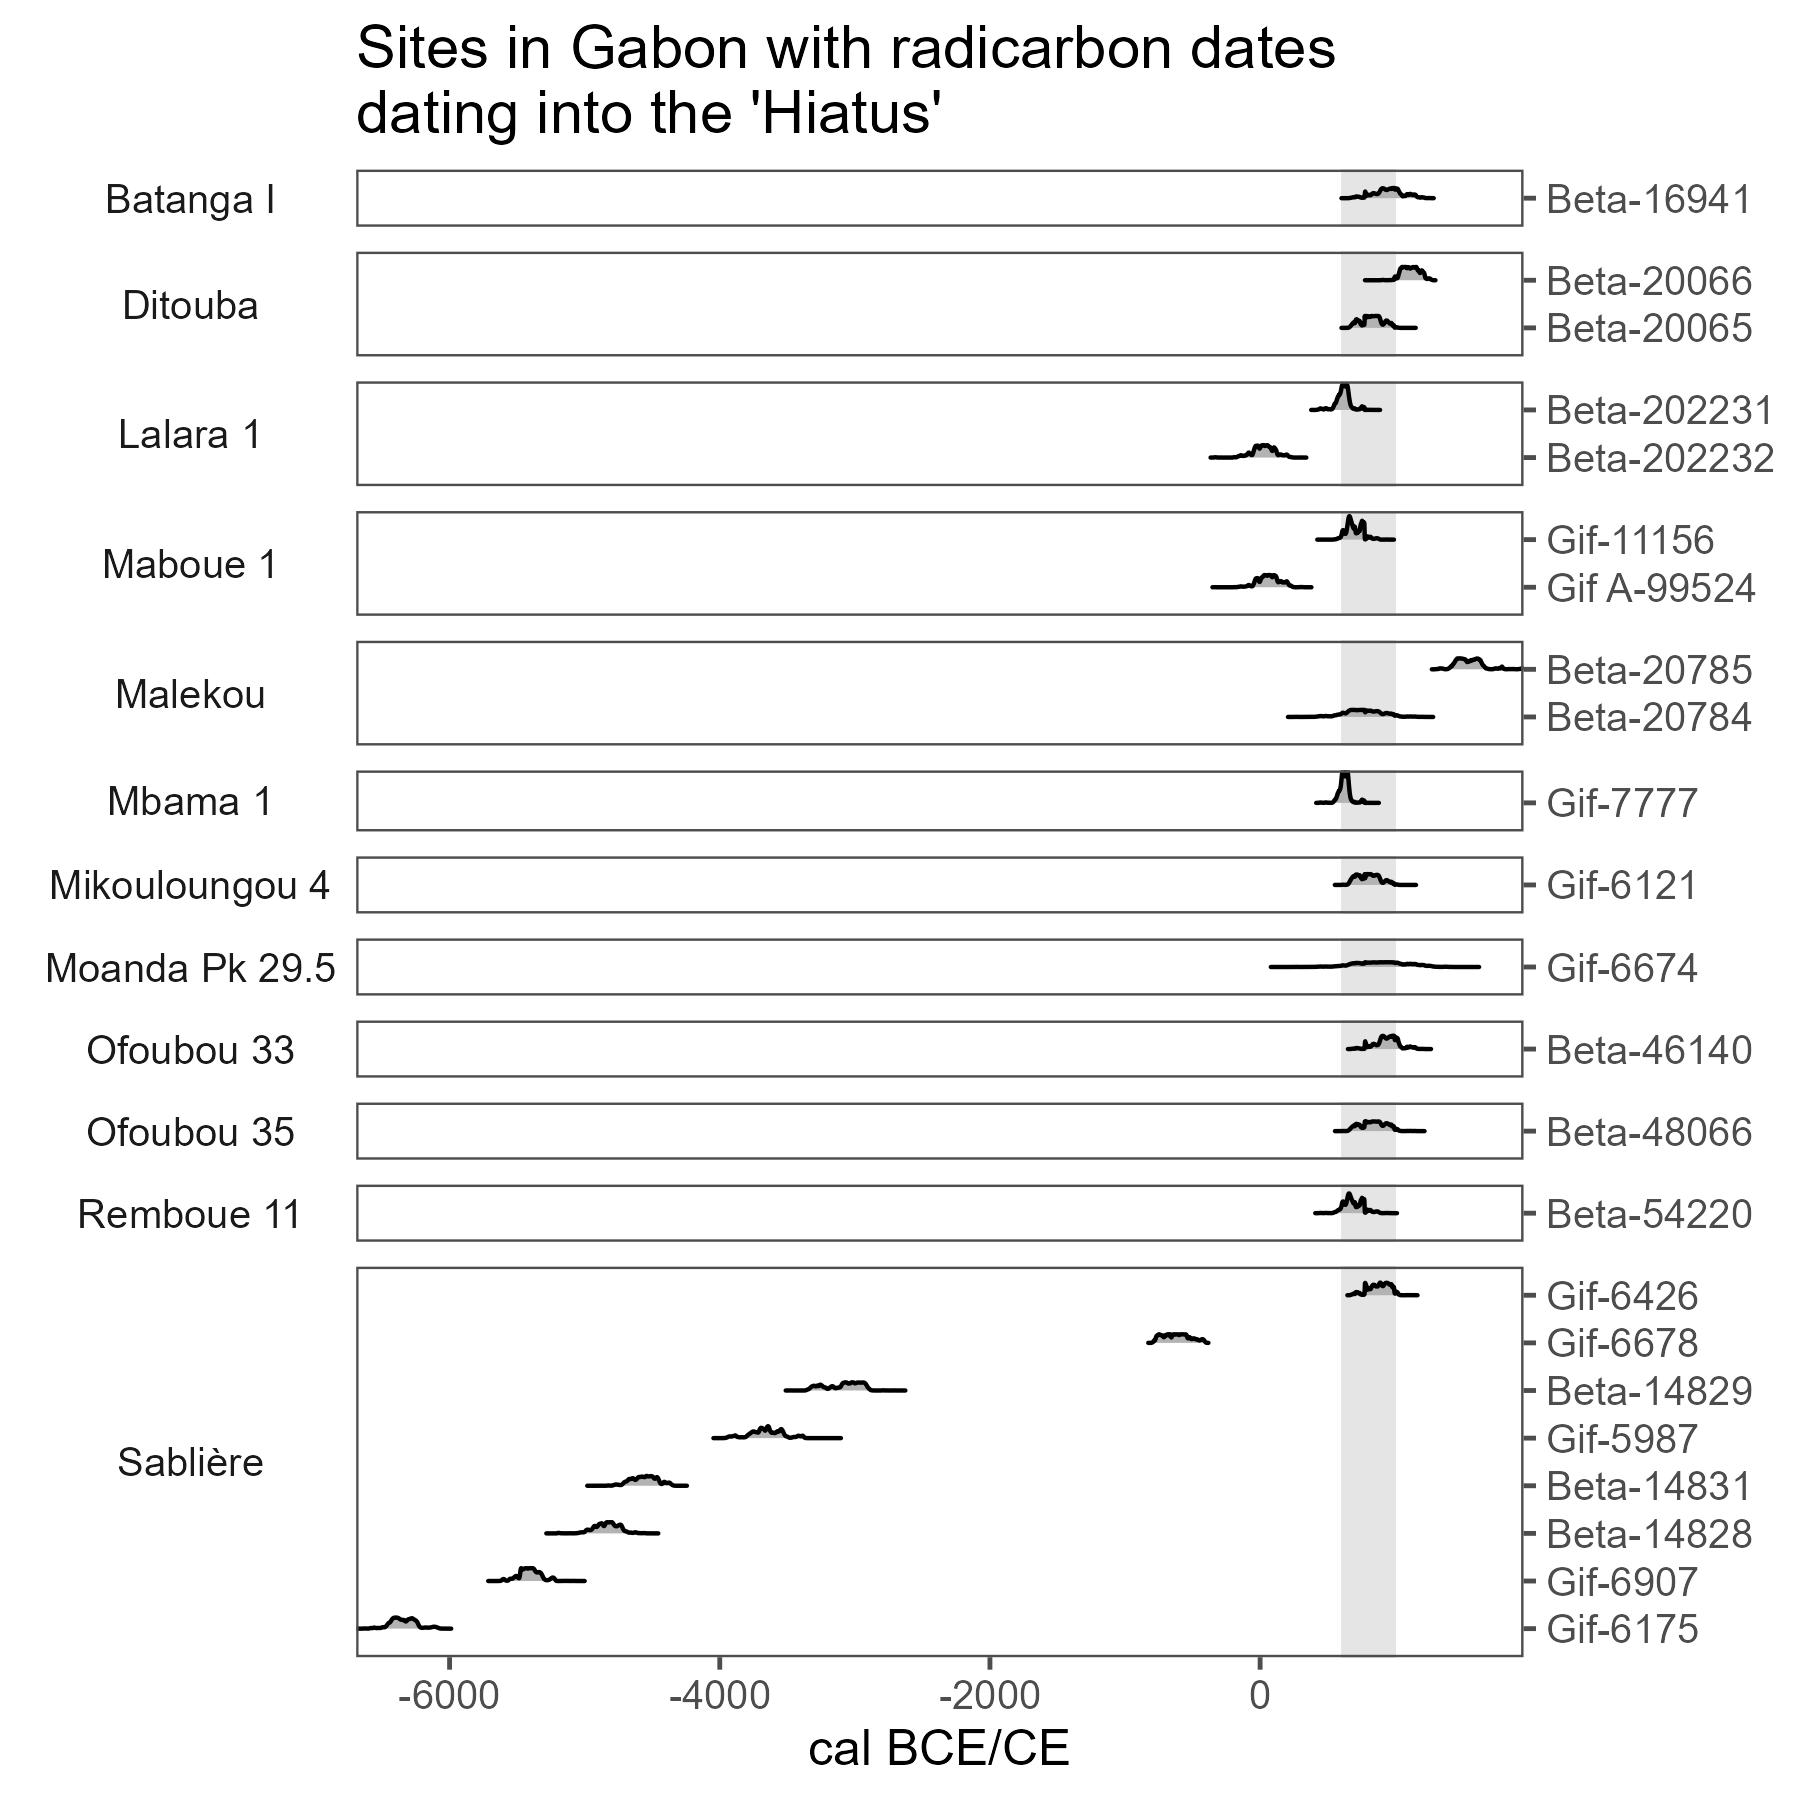
\includegraphics[width=\textwidth]{fig/varia_c14_hiatus_gabon_sites.jpg}
	\caption{Calibration of radiocarbon dates from archaeological sites in Gabon that yielded at least one date with the median age falling into the proposed 'hiatus' (grey shading) \citep{Seidensticker.2021e}.}
	\label{fig:14c_sites_gabon_hiatus}
\end{figure*}

\point 22) Middle Iron Age Hiatus in the Congo Basin (pages 25-26)

Lines 789-790: "an extensive reduction or nearly complete discontinuation of settlement activities was reported earlier for Gabon".

This is not correct as this argument has been challenged for Central Gabon and also because we have evidence of continuous settlements at least in North West Gabon.

\reply{The paragraph was rewritten. The sole critic of these findings -- the author is aware of -- is B. Clist. Concerning this debate the authors view is expressed above (see \ref{rev3:clist}). \citet[3, 6, 8, Fig. S4]{Seidensticker.2021e} clearly state that there are communities persisting throughout Central Africa, not refuting the general finding of a large-scale reduction in human activity. Concerning the sites with "evidence of continuous settlements", the author compiled all sites in Gabon with radiocarbon dates of which at least one date falls into the proposed 'hiatus' (Fig.~\ref{fig:14c_sites_gabon_hiatus}). Only the site of Sablière yielded more than two radiocarbon dates, most of which cover the early Holocene. Based on that, the author fails to fully comprehend the reviewers comment.}

\point Lines 791-793: Leka (2008) reported an interruption of settlement activities at sites north of Yaoundé (Cameroon) between the 1st and 10th century CE.

The results are preliminary. It is shown by the lack of radiocarbon dates during 10 centuries, a period far larger than the one the author suggests for his Middle Iron Age hiatus of some 3 centuries.

\reply{The results of Marie Juliette Leka were presented during the SAfA meeting 2008 in Frankfurt a.M. \citep{Leka.2008} and in her unpublished PhD thesis \citep{Leka.2013}. The author concurs with the reviewer that the results of Leka show an even more severe hiatus within the record of 14C dates than the poposed setback in human activity during the 6th to 10th century CE \citep{Seidensticker.2021e}. This reference was removed from the text due to the nature of the source and chronology as outlined by the reviewer.\label{rev3:leka}}

\point Lines 793-795: The Dibamba site in Cameroon is a single hilltop. It is common for any site to produce a settlement picture with large periods of inactivity. Three such periods are known on this site: c. 900-1600 cal BP (1050-350 CE), 1900-2400 cal BP (50 CE-450 BC) and before 2500 cal BP.

\reply{While a review of the available radiocarbon dates from Dibamba (Fig.~\ref{fig:14c_dibamba}) illustrates the multi-phased nature of the site, the lack of dates falling into the proposed setback in human activity during the 6th to 10th century CE \citep{Seidensticker.2021e} remains striking.}

\begin{figure*}[!tb]
	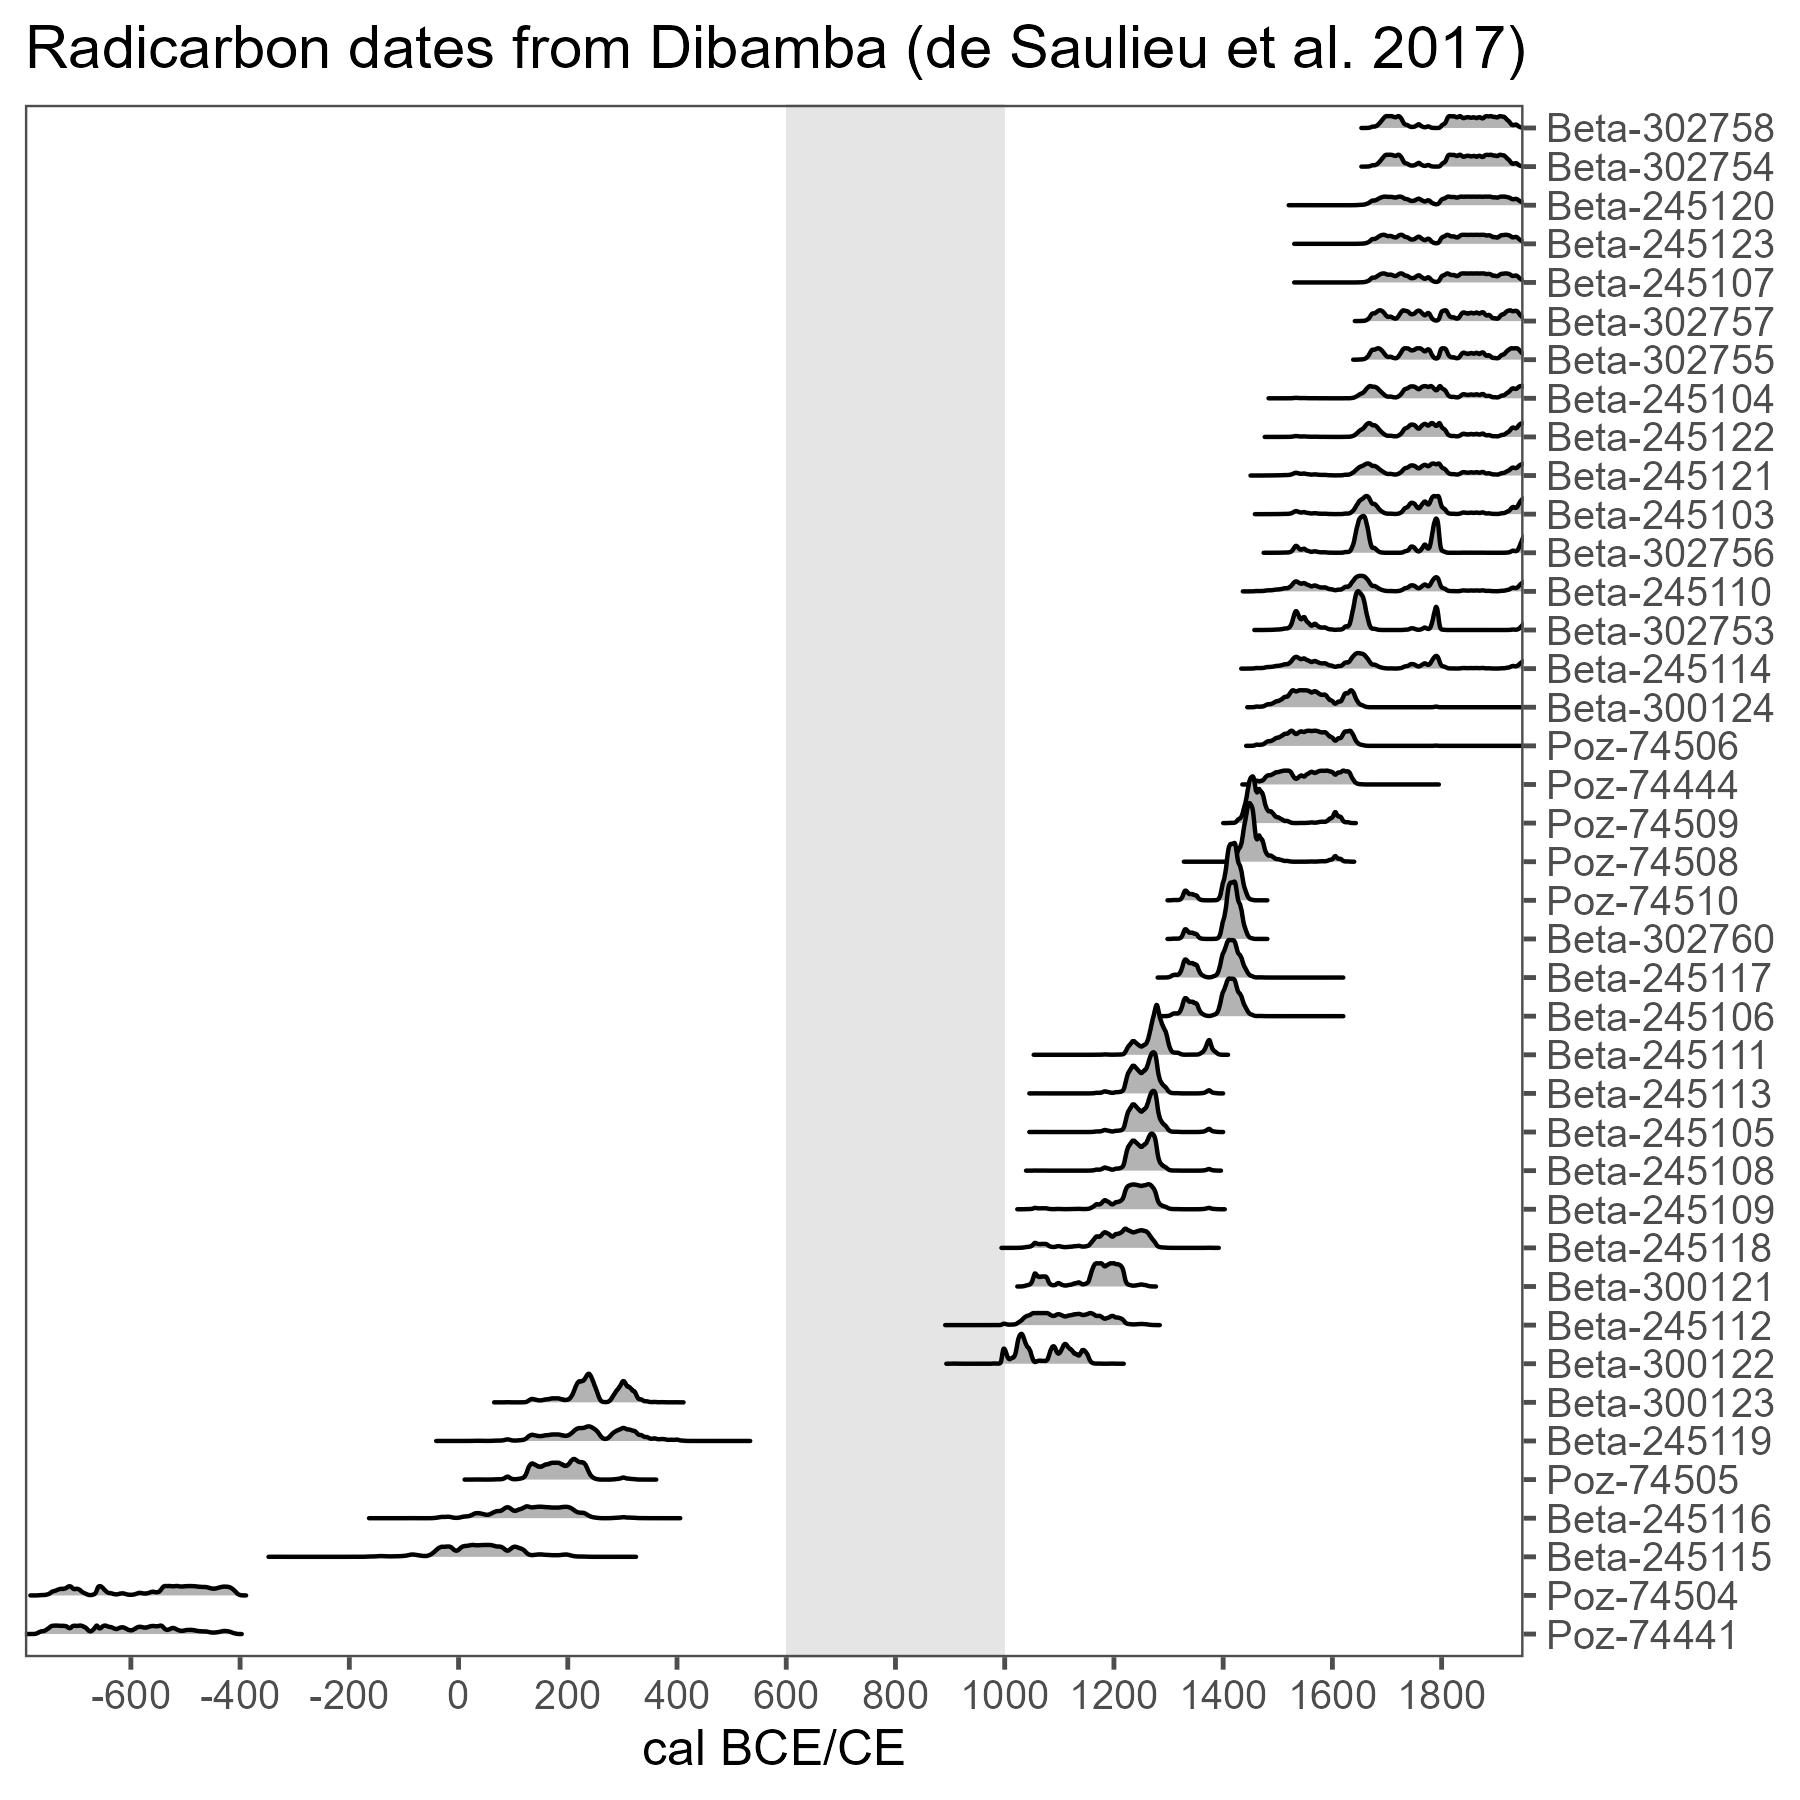
\includegraphics[width=\textwidth]{fig/varia_c14_dibamba.jpg}
	\caption{Carlibrated radiocarbon dates from the site of Dibamba \citep{Saulieu.2017} and the proposed setback in human activity during the 6th to 10th century CE \citep[grey shading;][]{Seidensticker.2021e}.}
	\label{fig:14c_dibamba}
\end{figure*}

\point Lines 795-800: Corisco is Corisco Island off the continent. On the continent, we find a continuous human occupation from the Okala Group to the Angondjé Group, from times BC until the time of the first Portuguese ships.

\reply{The authors understands the sequence of pottery groups in Gabon as follows \citep[Fig.~S1A "B) Gabon)]{Seidensticker.2021}: The start of the pottery sequence in Gabon is marked by the pottery group described by \citet[489--533]{Clist.20042005} as Okala group, after a site close to Libreville. \citet{Clist.20042005} integrates the earlier described pottery group Epona, which was found within the middle Ogooué valley \citep{Oslisly.1992,Oslisly.199495,Oslisly.1998,Oslisly.2001a,Oslisly.2001b}, as well as the Yindo pottery group of the Lopé reserve \citep{AssokoNdong.2000,AssokoNdong.2002}, into the Okala group. Okala pottery shows distinct similarities to the early pottery groups found within the coastal area of Cameroon. The available set of 14C-dates cover the 8th to 1st c. BCE. After the end of the Okala group, which is attested for within the entire north of Gabon and has strong links to groups from southern Cameroon, the pottery groups within Gabon shows a distinct regionalization, with three more or less contemporaneous groups. The Okanda group is distributed within the middle Ogooué valley and can be dated into the 5th c. BCE to 5th c. CE based on 14 14C-dates \citep[619--622]{Clist.20042005}. Otoumbi pottery is only attested for within the middle Ogooué valley, but slightly further north than the contemporaneuous Okanda group. The available 11 14C-dates indicate the 4th c. BCE to 6th c. CE as the time-period of the Otoumbi pottery \citep[623--625]{Clist.20042005}. Oveng pottery has been found within the area of Libreville \citep[614--618]{Clist.20042005} as well as the small island of Corisco \citep{GonzalezRuibal.2011,SanchezElipe.2015,SanchezElipe.2016}. The available 21 14C-dates associated with Oveng pottery are conclusively spaning the 1st to 6th c. CE, with only one date being slightly older and two dates slighly younger. A differentiation of the Oveng pottery into an early, middle and younger phase has been proposed for the inventories from Corisco island \citep{SanchezElipe.2015,SanchezElipe.2016}. Substantial evidence of the former ‘Group II’, as defined by \citep[628--631]{Clist.20042005}, have been discovered on the island of Corisco and the pottery group has been renamed Nandá \citep[357]{SanchezElipe.2015,SanchezElipe.2016}. Nandá pottery has -- up to now -- only to been found within the area of Libreville and on Corisco island. Ten 14C-dates indicate the 7th to 12th c. CE, with most dates being younger than 1000 CE. The successor of the Nandá pottery in the area of Libreville and Corscio island is the Angondjé group, which is associated with the first European contact finds and dates into the 10th to 16th c. CE \citep[357--358]{Clist.20042005,SanchezElipe.2015,SanchezElipe.2016}. In terms of vessel shapes and decorations, the author understands that the styles Okanda, Otoumbi and Oveng are derived from the Okala pottery, while Nandá vessels show quite different shapes and decorations \citep[212 Fig.~98]{Seidensticker.2021e}, thus indicating they are potentially part of a distinct tradition/line of development. This and the fact that the bulk of dates associated with Nandá pottery dates to later than the 10th century CE \citep[356--357]{SanchezElipe.2016}, let the author to the conclusion that the sequence of pottery groups in Gabon is not continuous.}

\point The examples the author chooses is similar to cherry-picking. The bigger trend mentioned Line 800 has been challenged in publications which are not referenced.

We need a serious discussion of the matter considering all the available publications on the matter, not limited to Seidensticker et al. 2021 and de Saulieu et al. 2021.

\reply{The listed individual examples are anecdotal evidence at best, while empirical data can only be derived from macro-level studies such as the ones performed by \citet{deSaulieu.2021a} and \citet{Seidensticker.2021}. Concerning this, please also see the last statements on \ref{rev3:clist}.}

\point The hiatus for the Inner Congo Basin is discussed from Lines 802 to 831. The text suggests a hiatus existed from the 6th to the 10th centuries CE. The demonstration is a flawed one because it relies on the availability of radiocarbon dates which are scarce all over the Congo Basin leaving most of the pottery styles undated.

How many dates do we have to pinpoint the Bokuma and Lingonda styles? Or the following Bondongo style?

\reply{The Bokuma pottery is considered to be contemporaneous to the Lingonda group \citep[120]{Wotzka.1995} and based on a single radiocarbon date from the eponymous site of Bokuma (GrN-14004), which is associated with Lingonda pottery as well, the style can be dated into the 3rd to the mid of the 6th c. CE for the time being. There are six radiocarbon dates associated with Lingonda pottery from the Inner Congo Basin. Based on the stylistic relations and derived chronological evidence, \citet[115]{Wotzka.1995} only accepts three to be representative for the Lingonda style (GrN-13076, GrN-14004, KN-4206). In general did \citet[115]{Wotzka.1995} consider the second half of the 3rd to the 7th c. CE the period of the Lingonda group. Besides the Imbonga style, the pottery of the Bondongo group is currently the most well-dated style within the Inner Congo Basin. Nine out of 14 radiocarbon dates that were associated with Bondongo pottery have been accepted by \citet[138 Tab.~58]{Wotzka.1995}. Those nine dates cover a period from the 11th to the end of the 14th c. CE.}

\point Lines 826-827: "… 'gap' or 'hiatus' within the sequence of the Inner Congo Basin that has been observed all over the Congo Basin"

Again, the proposal does not fit with the entire Congo basin as research has been limited to small areas of this vast expanse. See papers contradicting the author's position.

\reply{The statement has been amended to properly suit the cited literature.}

23) Conclusions:

\point Lines 886-887: "available data from the middle of the 1st millennium CE onwards must be considered incomplete".
And
Lines 881-883: "The settlement sequence of the northern and western Congo Basin sketched out within this study must, at least in part, be taken cautiously due to the limited sources available."

These statements from the manuscript's Conclusions sums up all our comments.

\point Lines 867-869. "… the prevailing hypothesis of the Sangha River Interval must be rejected from an archaeological perspective ". This statement must be developed, because as it is the reader cannot understand really what it means, he needs to go through the paper to uncover the section talking about it.

\reply{The statement was amended with the relevant references. Besides that, the manuscript devotes an entire section of the discussion to this issue.}

\point Line 870. The setback in human activity of the 7th-10th centuries must be questioned, the data at hand must be better put in perspective using the latest publications.

\reply{See \ref{rev3:clist}.}

\point Line 880. The Bobusa Group's existence and its dating has been questioned. See below. It cannot be kept in the conclusions.

\reply{The characteristics of the Bobusa group as outlines in the manuscript and \citet[162--165]{Seidensticker.2021e} are in such a way distinct from any other pottery found in the study area, that it can not be related to any other line of development or tradition.}

\point Under 'other finds' page 11, we read:

"Several vessels from a partially eroded pit on the banks of the Likwala-aux-Herbes (Kilometer 186) have no comparison in the region in terms of vessel shapes and decorations (Seidensticker 2021, 165-168, 339-340). Time constraints during fieldwork only allowed a quick sampling of the pit, obtaining a nearly complete vessel, four larger fragments and 13 smaller sherds (Eggert 1993, Fig. 16.15; Seidensticker 2021, Pl. 76.1-11). A charcoal sample dates this features between the 2nd century BCE to the 3rd century CE (KI-2893). The vessel has a flat base, convex belly, and a slightly elaborated shoulder leading to a concave neck and a flared rim. Its decoration consists of crudely made crossing grooves made with a comb on the shoulder and impressions beneath the rim. Further fragments show similar decorations. Overall, the vessel's shape is substantially different from those of the contemporaneous Pikunda-Munda style. Some aspects of the ceramics resemble a vessel found at Gbadolite on the upper Ubangi River (Eggert 1984, 277-278 Fig. 7). Nevertheless, the only accurate comparison for its shape, decoration technique and motives can be found among pottery of the Ngovo group in the lower Congo region (de Maret 1986)."

Reviewer's comments:

a) There is a single sample dated from a partially studied pit on the bank of a river, the result must be cautiously used especially when the associated pottery has no local connection (KI-2893: 1960+/-90 bp, mean calibrated date of 1861 cal BP, meaning it is much younger than the Ngovo Group, the date would fit with the start of the Kay Ladio Group or Style in Bas-Congo).

b) The comparison with the Ngovo Group the present reviewer knows very well, based on the illustration with 3 pots and sherds in Eggert 1993 is not at all convincing.

c) Looking at the Gbadolite pot in Eggert 1984 shows this vessel is strikingly different from the few illustrated pottery from the Eggert 1993 publication.

d) Looking at figure 76 in the 2021 edited PhD, none of the 11 pots or sherds have a relationship with the Ngovo Group.

e) Geography: as the crow flies the distance from the Likwala-aux-Herbes River to Bas-Congo is about 700 km, a bit too far away for any direct comparison.

Reviewer's conclusion: This means that the reviewer is convinced the connection proposed cannot be sustained and be incorporated in this text.

\reply{The inventory of the single pit at the bank of the Likwala-aux-Herbes river constitutes a singular find, with exceptional characteristics for its date. The features of the vessels originating in this pit can not be joined with other ceramics from the western Congo Basin. The author acknowledges that the reviewer opposes any reference to the Ngovo pottery of the Lower Congo. A direct comparison was included in \citet[118 Fnt.~152; Fig.~\ref{fig:lkw186_ngovo}]{Seidensticker.2021e}. Besides the present case, the author found four more cases of supra-regional comparisons between pottery of the northern and western Congo Basin: the discussed similarities between the Ngbanja style and the pottery of the Early Phase of the Kisangani area (see \ref{rev3:ngbanja}), the Bokonongo style, which shows similar shapes and decorations patterns as the Oveng pottery of Gabon (see \ref{rev3:bokonogo}), the case of the Bobusa pottery which is superficially reminiscent of the pottery known from the Kinshasa region \ref{rev3:bobusa}, and the observation that Pikunda-Munda vessels show comparative features to the pottery excavated at Yatou, on the mouth of the Sanaga river in Cameroon \citep[118 Fnt.~152]{Eggert.2002,Seidensticker.2021e}. The statements in the text were diminished. The author is convinced that research into supra-regional connections between ceramics in Central Africa can be conducted in a reproducible fashion following the approach outlined above (see \ref{rev3:ngbanja} \& Fig.~\ref{fig:potterystyles_eia_attributes_ca}) and in consequence will illuminate putative -- but as the author sees -- slowly emerging supra-regional networks.\label{rev3:lkw186}}

\begin{figure*}[!tb]
	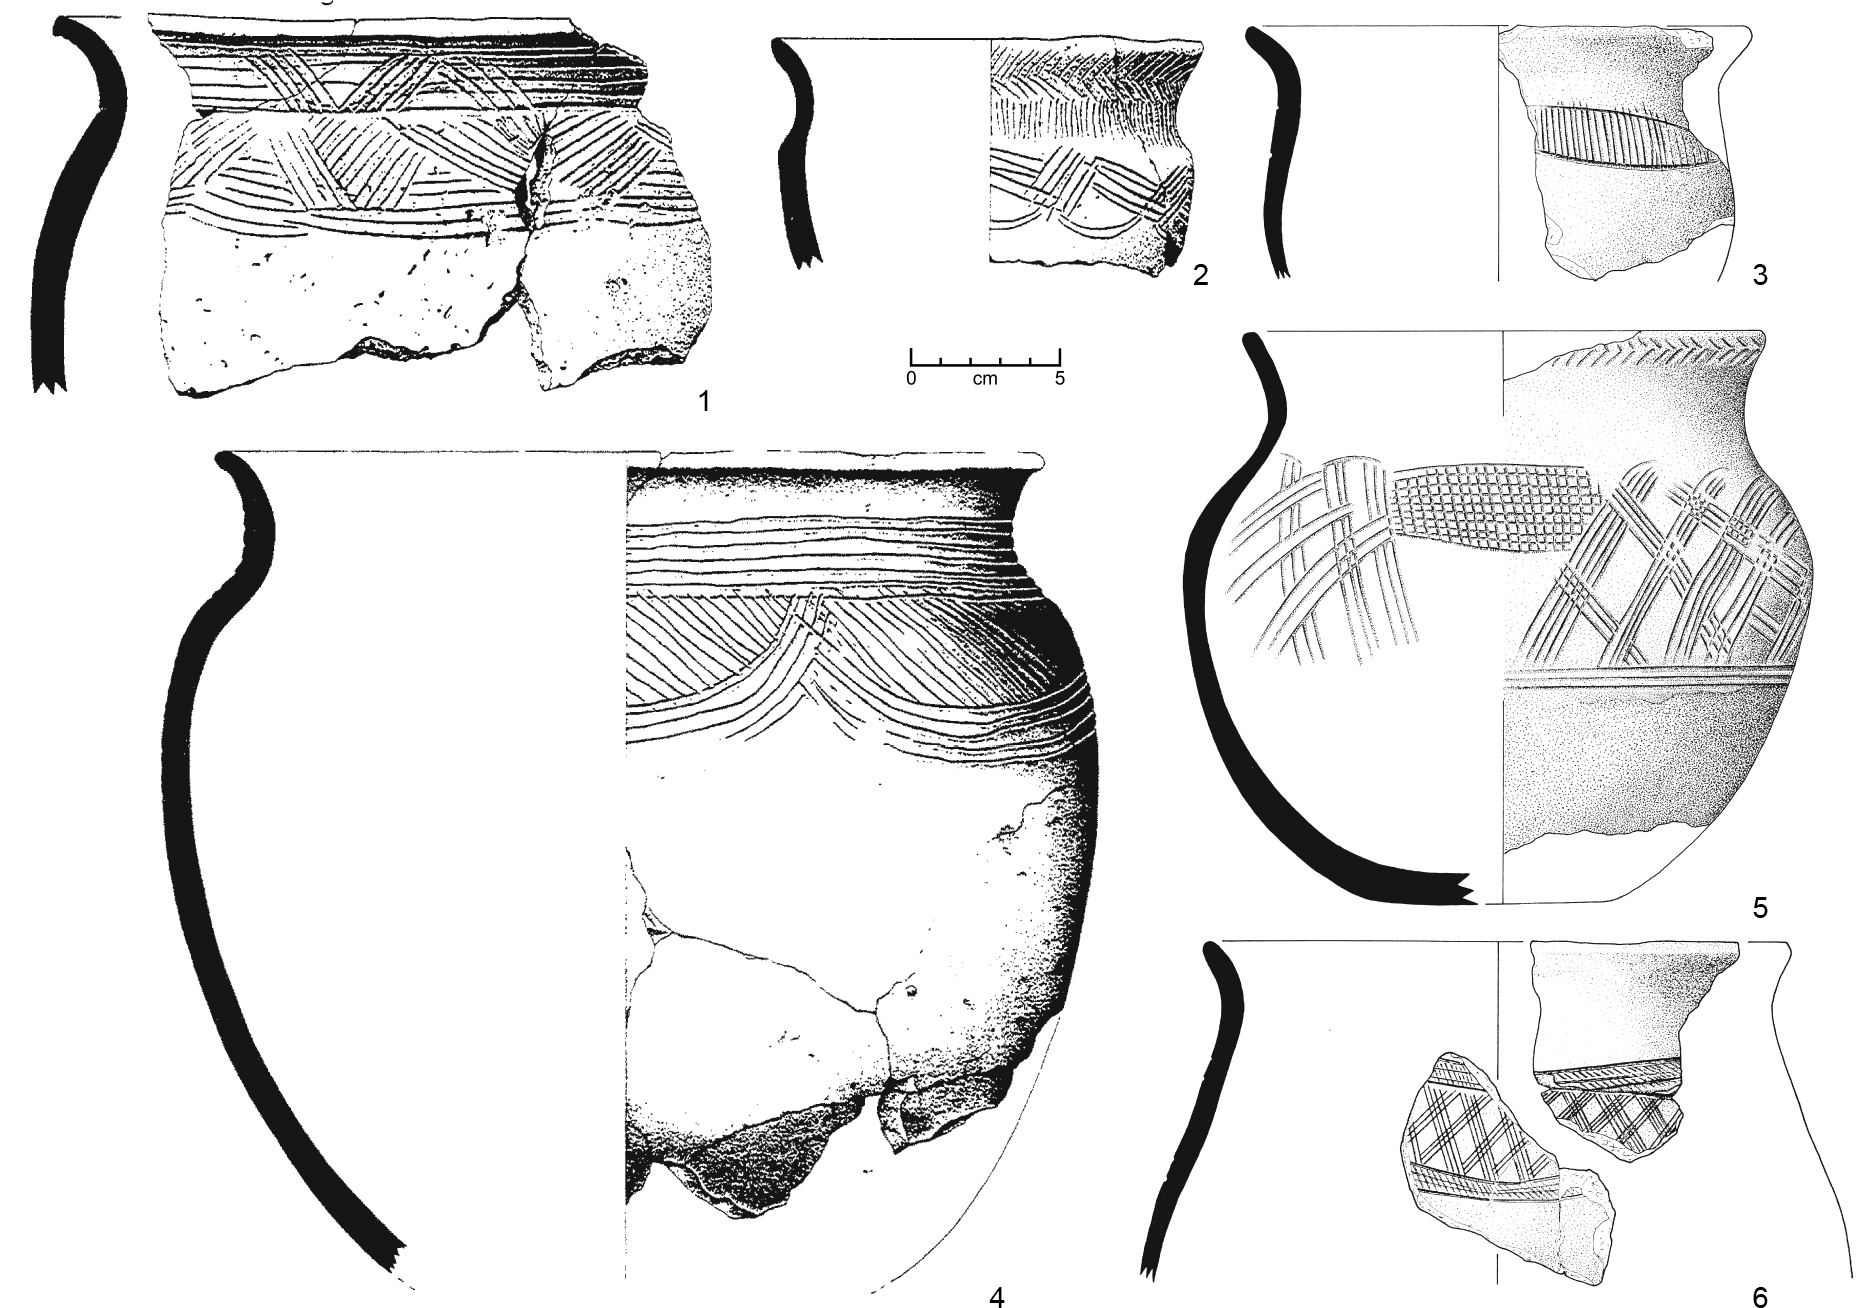
\includegraphics[width=\textwidth]{fig/Ngovo-Typen.jpg}
	\caption{Pottery of the Ngovo style (1--2, 4) and from the pit feature LKW~87/186 at the Likwala-aux-Herbes river (3, 5--6) illustrating the superficially similarities such as: flat bases, convex bellies, and a slightly elaborated shoulder leading to a concave neck and a flared rim, decoration consisting of crudely made crossing grooves made with a comb on the shoulder and impressions beneath the rim. Sources: 1: \citet[108 Fig.~4.7]{deMaret.1986}; 2: (ibid. 108 Fig. 4.14); 3: \citet[Pl.~76.2]{Seidensticker.2021e}; 4: \citet[111 Fig.~5.3]{deMaret.1986}; 5: \citet[Pl.~76.1]{Seidensticker.2021e} ; 6: (ibid. Pl.~76.3).}
	\label{fig:lkw186_ngovo}
\end{figure*}

\point Another problem lies with another find (pages 11-12):

"The Bokonongo style is an interim term for an inventory of 19 vessel units from seven sites, including Pikunda on the middle Sangha River, that show very distinct characteristics: all vessels are either rather tall with convex bellies and concave necks ending in cylindrical rims or bowls with inverted rims (Fig. 3.4; Seidensticker 2021, 120-123). Decorations consist of grooves beneath the rim and on the neck and shoulders, mainly forming horizontal, chevron or crossing motives. About half of the inventory showed a fabric similar to that of the Pikunda-Munda group, while a quarter showed grog tempering. At the same time, the remainder contained a heterogenous mix of quartz and grog. All finds are surface finds and not associated with any indications of their dating. The only accurate comparison in terms of morphological characteristics and decorations can be found among the Oveng pottery found in north-western Gabon (Clist 2004, 615-618) and on the island of Corisco (Equatorial Guinea) (Gonzalez-Ruibal et al 2011; 2012; Sanchez-Elipe 2015, 217-221; Sanchez-Elipe et al 2016, 351-355). Oveng ceramics date from the 2nd century BCE to the 5th century CE (Clist 2004, 555 Fig. 7-14). The resemblance provides a provisional chronological estimate for the Bokonongo pottery to date around the first half of the 1st millennium CE (Fig. 6)."

Reviewer's comments:

a) We have a style defined from surface finds coming from 7 sites established along the Sangha River and downstream to the Congo River (see Abbildung 51, page 123 of edited PhD 2021),

b) The fabric of the series as described is very heterogenous, unfit from a series coming from a common pottery tradition.

c) How can we be sure the potsherds represent contemporaneous deposits which eroded out of their original contexts?

d) The only comparison found is with the Oveng style regarding shapes and decoration. Out of the 3 shapes to be found in Seidensticker 2021 (book form of the PhD, see page 122, Abbildung 50), only one does have quite a similarity with one of the pottery shapes of the Oveng production, though strictly speaking the profiles are different. Can it be the so-called "Bokonongo style" developed such lip shapes to accept lids which are unknown by Oveng potters?

e) Furthermore, the decoration and other shapes from both styles does not have any similarities whatsoever. Within this "Bokonongo" style it is surprising to see such divergent types of pots.

f)  Inland and in Gabon, near to the Oveng style using communities, we find the Otoumbi and Okanda Early Iron Age Groups with which no connection is found with Bokonongo though they lie in between Oveng and Bokonongo. Okanda pottery users were connected with Oveng as is evidenced by an Okanda pot found in an Oveng context.

The Oveng Group is understood as pottery-users and fishermen settling along the coast up to south of the Ogooué river in Gabon without moving to the east deep inside the forest; exchanges though existed between central Gabon and the coast along 200 km of forest as evidenced by the Okanda pot found on the coast.

g) The accepted chronology for the Oveng production proposed here is wrong. The oldest accepted date is c. 1,970 BP. The older dates are from shells, which date older than the charcoal-based ones.

Reviewer's conclusion: This means the connection proposed cannot be sustained and be incorporated in this text, and above all the chronology of Oveng cannot be superimposed on the Bokonongo pottery. The latter must remain undated until features of the style is properly excavated. Maximum a passing reference to a vague similarity regarding the lip and neck shape of one type of pot can be kept.

\reply{The conclusions have been attenuated. Concerning comment b): The authors acknowledges the disparity in terms of macroscopic fabrics and thus considerable differences in the \textit{chaînes opéroires}, but wants add that we do know nothing about the structure of past pottery communities of practice in the Congo Basin. While there are ethnographic reports of centralized production, like in the main potters' village of Ikenge on the Ruki \citep{Eggert.1980c}, \citet[188]{Wotzka.1995} also reports that pottery produced in the two villages Ilemba and Bokonda (both near Boende), as well as in others on a much smaller scale, can be subsumed to the same style, leaving the possibility for local production. The author currently works towards a first approach to distinguish the local, intermediate, or trans-local nature of pottery in the Congo Basin by means of petrographic and geo-chemical analyses. Concerning comment d): Lids are also not reported from the the finds from the western Congo Basin. Concerning comment g) the text was amended. The oldest date not obtained by dating shell fragments is Beta-296117 (1940$\pm$40~BP) from Nandá (Fig.~\ref{fig:14c_oveng}).}

\begin{figure*}[!tb]
	\begin{subfigure}[t]{.38\textwidth}
		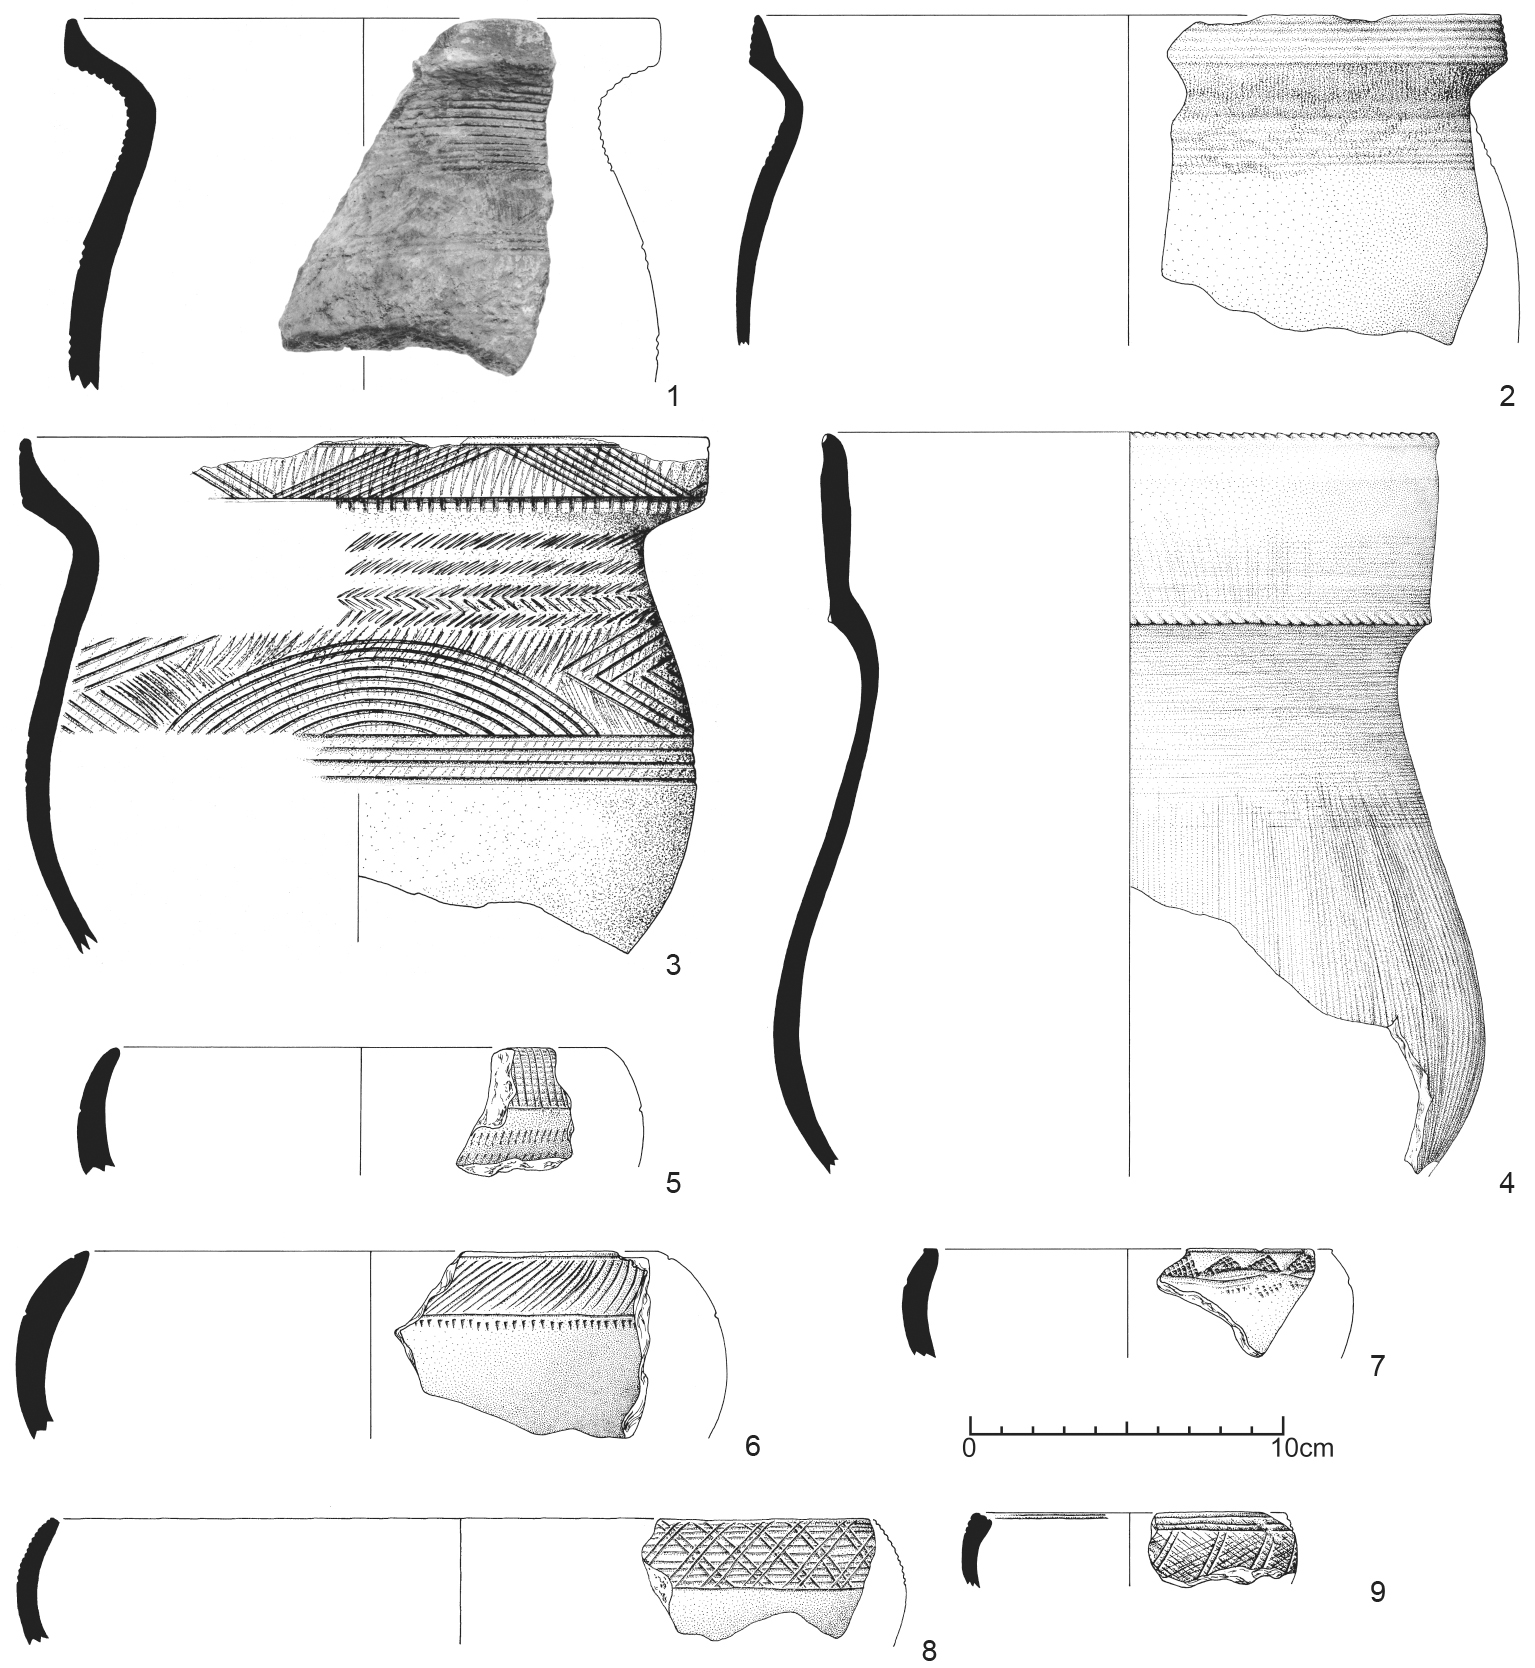
\includegraphics[width=\textwidth]{fig/BOG-Typen.jpg}
		\caption{Bokonongo pottery \citep[122 Fig.~50]{Seidensticker.2021e}.}
	\end{subfigure}\hspace{.5em}\hfill
	\begin{subfigure}[t]{.61\textwidth}
		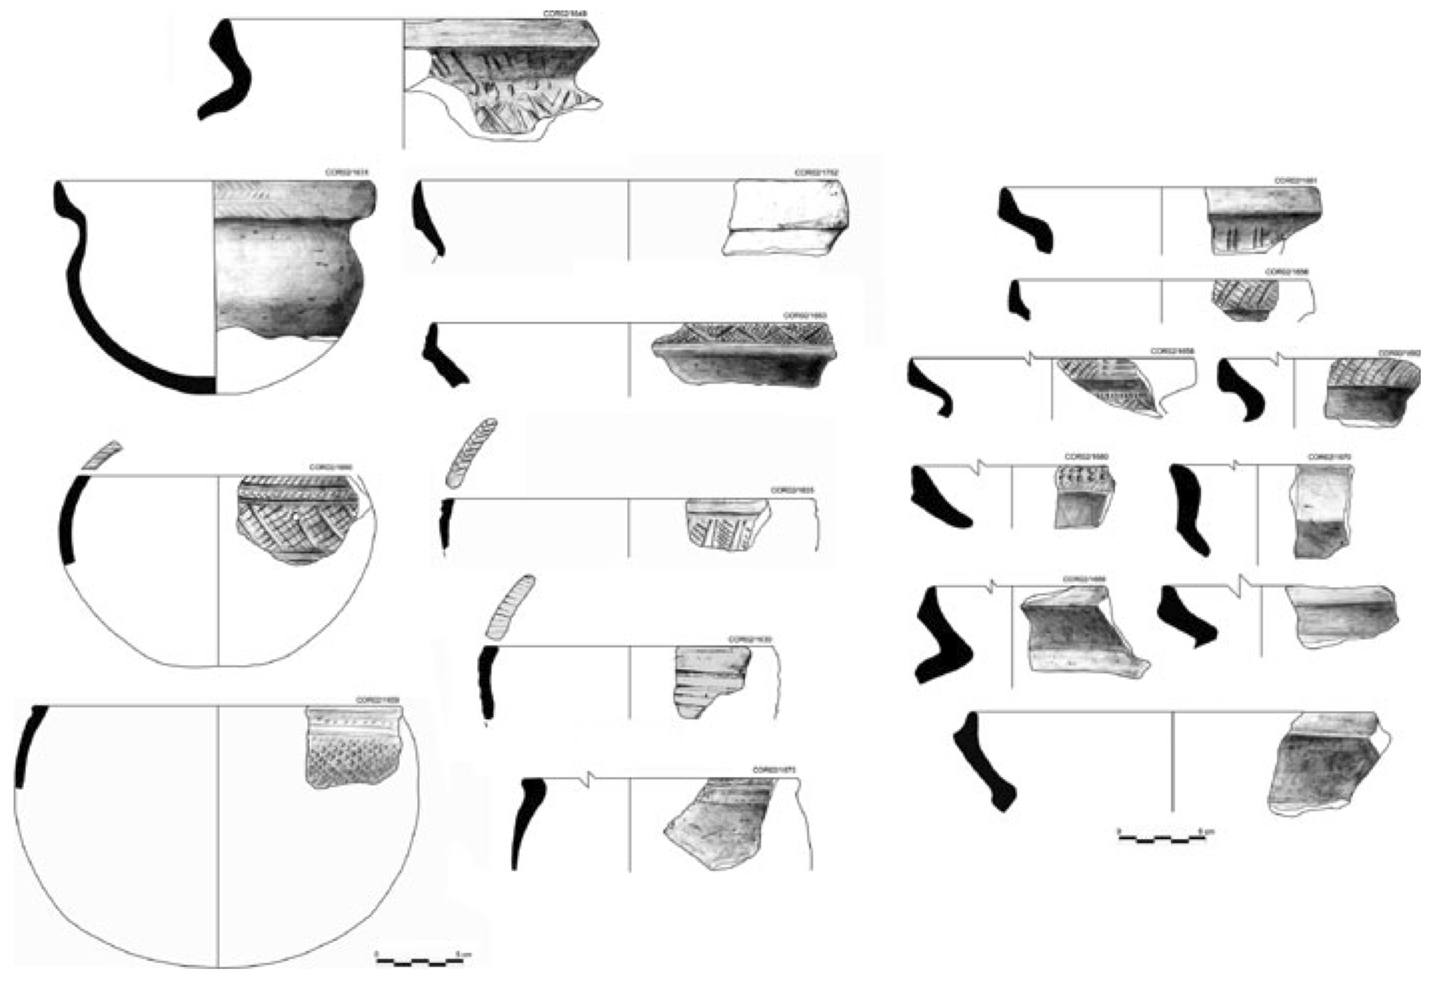
\includegraphics[width=\textwidth]{fig/GonzalesRuibal2012_134Fig15_Oveng-Trad.jpg}
		\caption{Oveng pottery \citep[134 Fig.~15]{GonzalesRuibal.2012}.}
	\end{subfigure}
	\caption{Comparison between the pottery provisionally summarized as Bokonongo style (a) and the Oveng group of Gabon (b).}
	\label{fig:vgl_bog_oveng}
\end{figure*}

\begin{figure*}[!tb]
	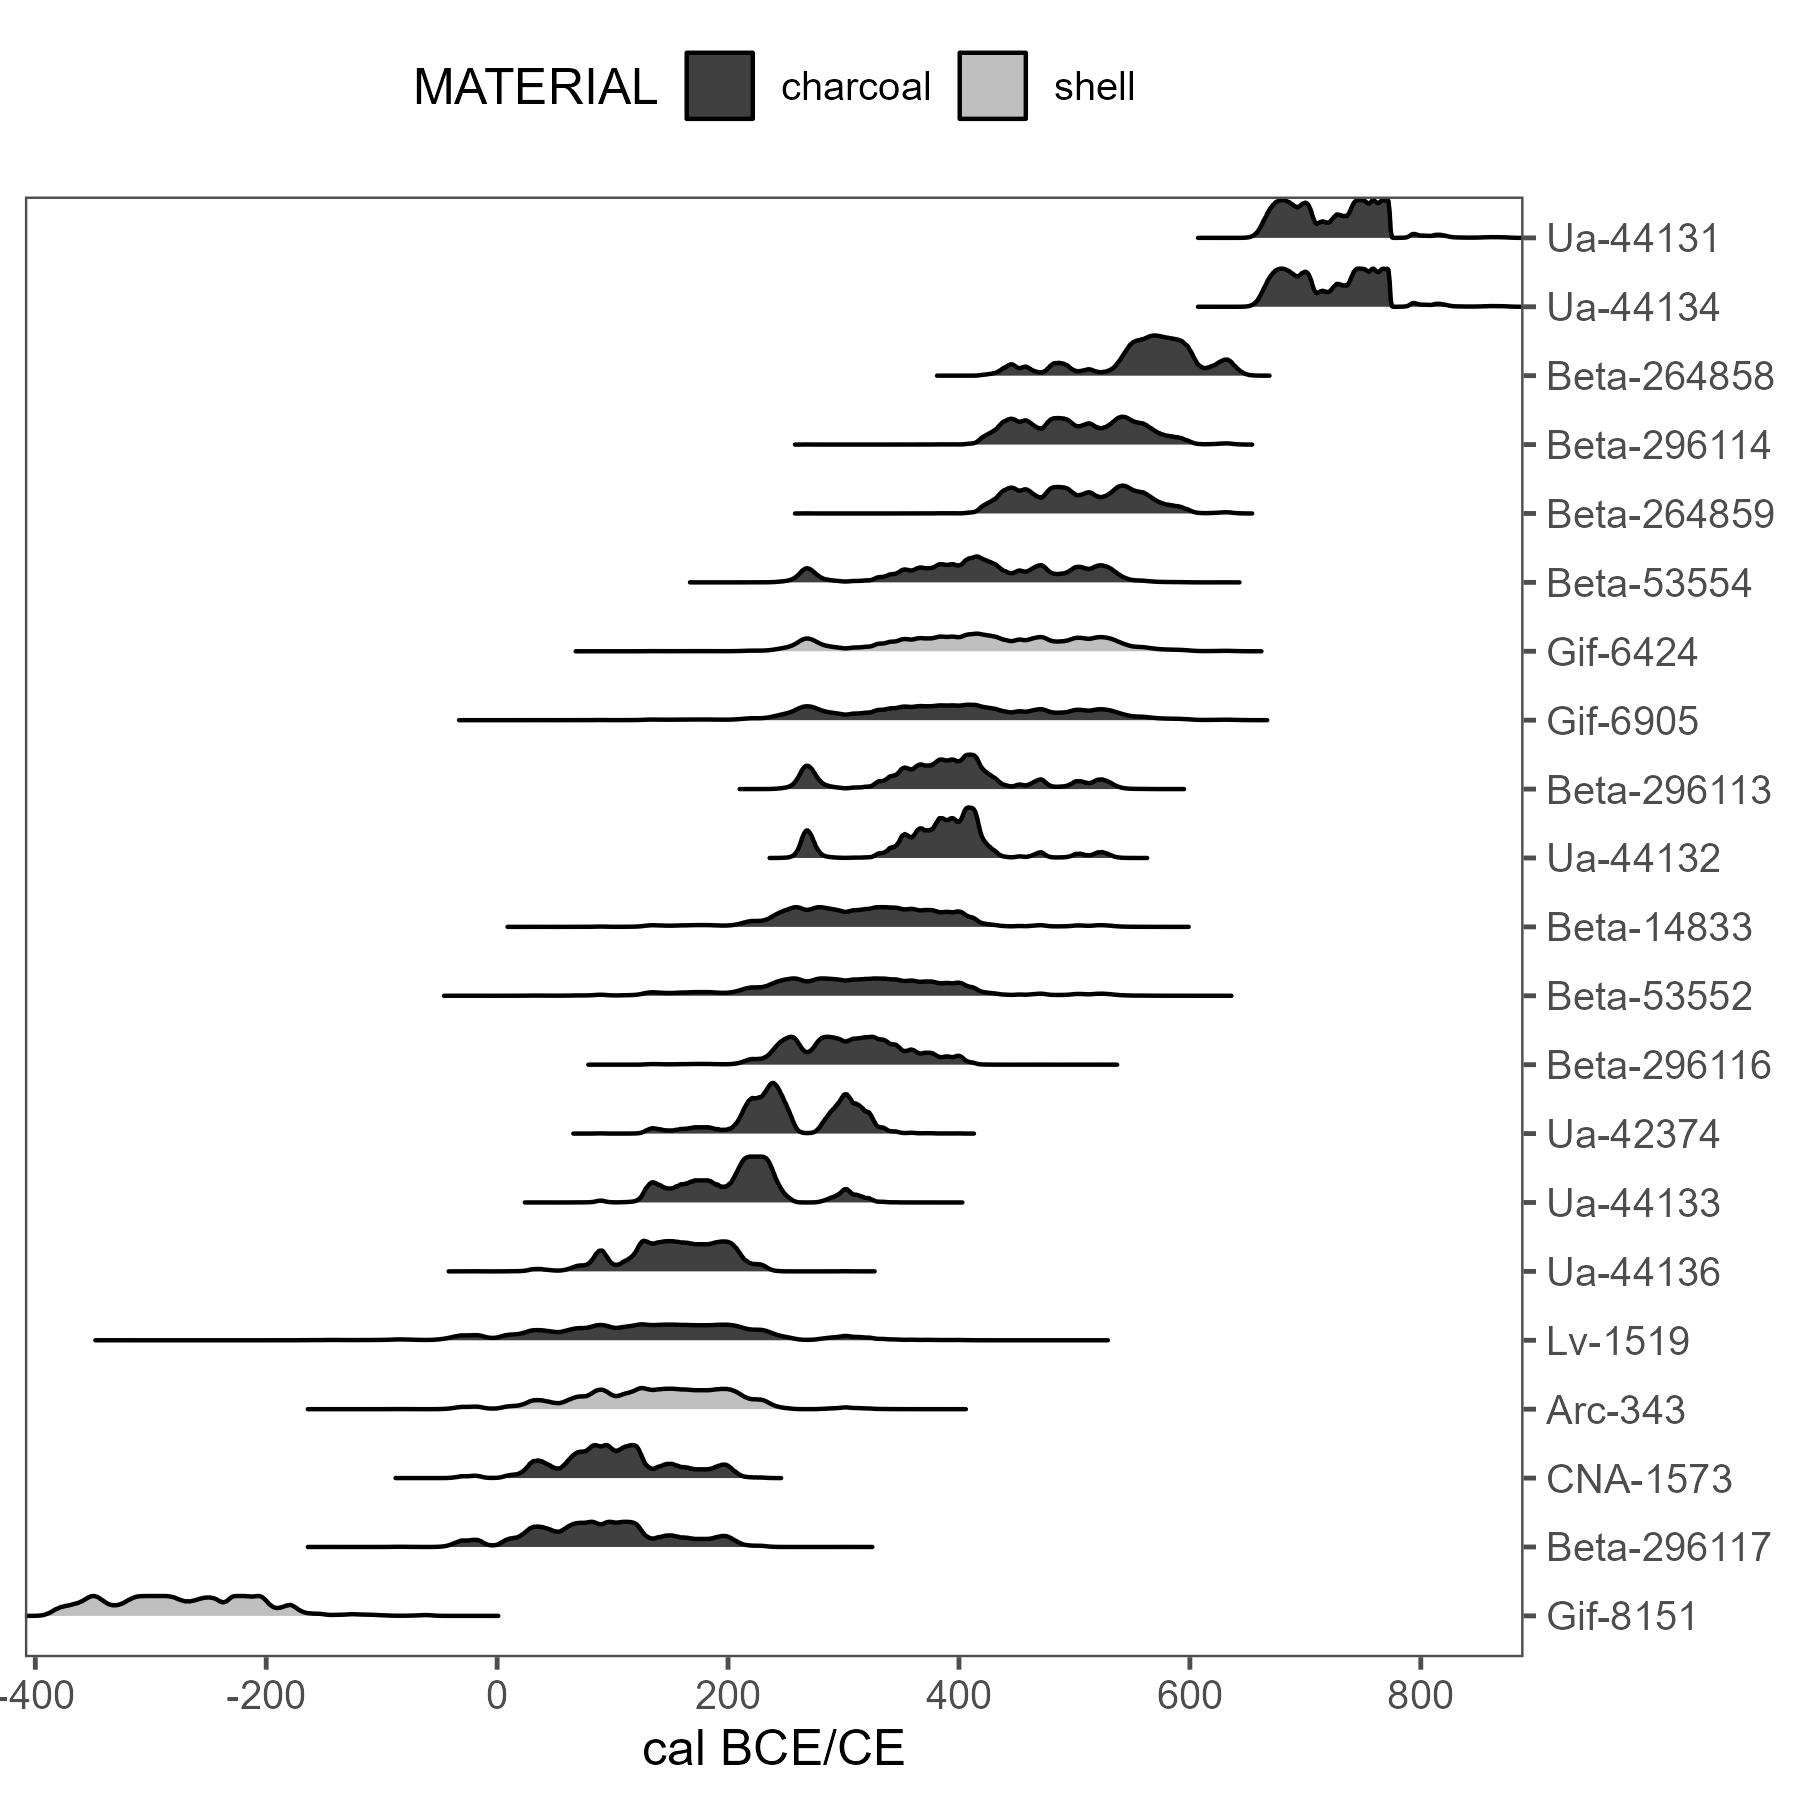
\includegraphics[width=\textwidth]{fig/varia_c14_oveng.jpg}
	\caption{Calibrated radiocarbon dates associated with Oveng style pottery derived of \citet{Seidensticker.2021f}.}
	\label{fig:14c_oveng}
\end{figure*}

\point A third and last example of "other finds" is about the Bobusa style, page 12:

"Close to the mouth of the Sangha River, in the very south of the study area, a unique kind of pottery was found that is characterized by predominant grog tempering and small globular pots with short everted rims or convex bowls with slightly inverted rims (Fig. 3.5-7; Seidensticker 2021, 162-165). This group is named after the site of Bobusa, located near the mouth of the Sangha River. While there are no radiocarbon dates available for this pottery
group, some of its characteristics show similarities to pottery found on the Ile des Mimosas in Kinshasa that is dated into the 2nd to 4th centuries CE (Eggert 1984, 279-280). This time span is provisionally also proposed as the age of the Bobusa pottery (Fig. 6)."

Reviewer's comments:
In the edited PhD, the Abbildung 79 (page 164) illustrates the position of the 6 sites where Bobusa style pottery was found, along the banks of the Congo River and the last part of the Sangha River slightly upstream. Some of the finds are illustrated on Abbildung 78, page 163.

We read that "some of its characteristics" link it up to pottery found at Kinshasa.

Indeed, some of the intact pots found on the Ile des Mimosas were illustrated by Eggert in 1984 and he associated to them a radiocarbon date.

a) Facts show the date of Kinshasa cannot be associated to the series of intact pottery still to be found in the archaeology museum of Kinshasa university; the date related to a "layer" with wood charcoal (some dated) and some undescribed potsherds. Not intact pots. These must have been found in unidentified burials as known elsewhere in Central Africa (Equatorial Guinea, Gabon, DRC-Katanga). The intact pottery from Ile des Mimosas consists of at least three series, probably slightly differing as their chronology, from differing burials. We need new finds from in and around Kinshasa to make the connection to the intact vessels.

b) Looking at the illustrations of some potsherds in Seidensticker 2021 and the few illustrated and intact pots in Eggert 1984, one cannot see any relationship.

c) In the edited PhD, page 163, one reads that "a characteristic feature of the Bobusa pottery is the occurrence of remains of red painting". In Bas-Congo remains of painting, also red, only happens on pots and clay tobacco pipes of the last centuries.

Reviewer's conclusion: It follows the so-called Bobusa pottery must remain undated and any relationship with Kinshasa removed from the paper.

\reply{Many thanks for the additional details concerning the finds from the Île des Mimosas. The author would be delighted to gain knowledge about a published source concerning this review of the site and its findings. Also many thanks for the note concerning the use of red painting. For the sake of this paper, the statements in text have been attenuated.\label{rev3:bobusa}}

Typos:
\point In table 2, to read conventional instead of convetional.

\reply{The table can now be found in the OSM and the typo has been corrected.}

\point Page 4, lines 23-24, it should read "the south-western parts of the Central African Republic".

\reply{The typo was corrected. Many thanks for spotting this.}

References:
\point 1) For Ndanga et al 2010 mentioned on page 12 we find in the reference section this:

Ndanga AJP, Cornelissen E, Lanfranchi R (2010) Quel lien entre les ateliers de taille de Ngo
Tchororo et la céramique de Batalimo (RCA)? / Stone knappers at Ngo Tchororo and pottery makers at Batalimo (CRA), did they meet?

Obviously, the reference must be completed.

\reply{The references was corrected.}

\point 2) Same problem here :

Leka MJ (2008) Nouvelles recherches archeologiques en pays Tikar: Premiers resultats

The study seems not to have been published.

\reply{Also this references was amended.}

\point Concluding recommendations and suggestions:

1) It would be better to extract all the technical descriptions about pot making, setting them up in a specific section, and showing how they changed through time and according to the geography of the Congo basin.

2) It would be better to rewrite the other sections, without the technical points, focusing on shapes and decoration from well dated (radiocarbon) styles.

3) Only after this, one can insert the other styles based on personal feelings about typological connections.

\reply{The author thanks the reviewer for these suggestions. A goal of this paper is to give readers a comprehensible overview of the edited PhD thesis \citet{Seidensticker.2021e} that was written in German. Thus, the structure of the paper and the way in which the data is presented, is intended to stay close to \citet{Seidensticker.2021e}. A structure as the one proposed by the reviewer would make sense as soon as the current work on the pottery technology of the Congo Basin is past the preliminary stage it is in right now (see~\ref{rev3:pottery_tech}).}

\end{reviewer}

%\bibliographystyle{spbasic}
\bibliography{references.bib}

\end{document}
